\documentclass[11pt]{report}
\usepackage{amsmath, bm}
\usepackage{stackengine}
\usepackage{graphicx}
\usepackage{caption}
\usepackage[titletoc]{appendix}
\usepackage{subcaption}
\usepackage{breqn}

\stackMath

	\addtolength{\oddsidemargin}{-.875in}
	\addtolength{\evensidemargin}{-.875in}
	\addtolength{\textwidth}{1.75in}

	\addtolength{\topmargin}{-.875in}
	\addtolength{\textheight}{1.75in}

\DeclareMathOperator{\diag}{diag}

\makeatletter
\def\@makechapterhead#1{%
  \vspace*{50\p@}%
  {\parindent \z@ \raggedright \normalfont
    \interlinepenalty\@M
    \Huge\bfseries  \thechapter.\quad #1\par\nobreak
    \vskip 40\p@
  }}
\makeatother

\graphicspath{ {figures/} }
\allowdisplaybreaks

\begin{document}
\tableofcontents

\chapter{Problem Statement}
Consider a 2-D strip of material that has infinite length, but finite thickness. The strip is constrained along its bottom surface by rollers, as shown in Figure \ref{fig:stripFig}.
\begin{figure}[h]
	\begin{center}
		\includegraphics[scale=0.7]{compressed_strip_drawing}
	\end{center}
	\captionsetup{format=hang}
	\caption{Diagram of the strip with finite thickness of $L$ in the $x_2$ direction, and infinite width in the $x_1$ direction. Rollers constrain the displacement in the $x_2$ direction on the bottom horizontal surface to zero. The displacement control sets the average stretch in the $x_1$ direction as $\lambda_1$.}
	\label{fig:stripFig}
\end{figure}

The displacement control problem will be considered. The average stretch in the $x_1$ is defined as $\lambda_1$. The loading parameter $\lambda$ will be defined as:
\begin{equation}
\lambda = 1 - \lambda_1,
\end{equation}
where a value of $\lambda = 0$ corresponds to no displacement. The problem will be restricted to only the compressive case, where $ 0 \leq \lambda < 1 $.

A compressible 2-D Neo-Hookean stored energy function $W$ will be used. It has the form:
\begin{equation} \label{eq:energyFunction}
W=\mu(x_2)\left[\frac{1}{2}(I_1 - 2- \ln{I_2}) + \frac{\nu}{1-\nu}(\sqrt{I_2} - 1)^2\right],
\end{equation}
where $\nu$ is a constant material parameter, and $\mu(x_2)$ is a material parameter that only varies in the $x_2$ direction. $I_1$ and $I_2$ are the principle invariants of the Cauchy-Green tensor $\mathbf{C}$ given by:
\begin{equation} \label{eq:I_functions}
I_1 = \mathrm{tr}\mathbf{C} \qquad I_2 = \mathrm{det} \mathbf{C}.
\end{equation}
The principle solution is simply a uniform squishing, with a deformation gradient constant throughout the domain. In an orthonormal basis alingned with the $x_1$ and $x_2$ axis, this is $F = \diag[\lambda_1, \lambda_2]$, where $\lambda_2$ can be solved from the quadratic:
\begin{equation}
\lambda_2^2 - 1 + \frac{2\nu}{1 - \nu}(\lambda_1^2 \lambda_2^2 - \lambda_1\lambda_2) = 0.
\end{equation}
A derivation of the principle solution can be found in Appendix \ref{append_principle}.

\chapter{Exponential $\mu(x_2)$}
The first case that will be considered is when the paramter $\mu(x_2)$ exponentially increases in the positive $x_2$ direction. Thus, it is of the form:
\begin{equation} \label{eq:mu_ex}
\mu(x_2) = \mu_0 e^{\kappa x_2},
\end{equation}
where $\kappa$ is the exponential growth parameter and $\mu_0$ can be taken as unity from scaling arguments.

\section{Initial Bifurcation}
By setting the second variation to go singular at the unstable mode and by separating the resulting linear PDE (Appendix \ref{append_first_sol}), the first birfurcated solution is of the form:
\begin{equation} \label{eq:first_bif_modes}
\mathcal{A}^2 =
\left \{
\begin{aligned}
  \overset{1}{u}_1 &= -v_1(x_2)\sin(\omega x_1) \\
  \overset{1}{u}_2 &=  v_2(x_2)\cos(\omega x_1)
\end{aligned}
\right \} , \qquad
\mathcal{S}^2 =
\left \{
\begin{aligned}
  \overset{1}{u}_1 &= v_1(x_2)\cos(\omega x_1) - v_1(0) \\
  \overset{1}{u}_2 &=  v_2(x_2)\sin(\omega x_1)
\end{aligned}
\right \},
\end{equation}
where $\mathcal{A}^2$ and $\mathcal{S}^2$ denote the symmetric and antisymmetric $u_1$ modes about the $x_2$ axis, respectfully. $\omega$ is an arbitrary constant that arises from the separation of the system of linear PDE's, and is realted to the wavelength of the instable mode. The $x_2$ dependence is:
\begin{equation}
v_1(x_2) = \sum_{i = 1}^{4}A_ie^{\alpha_i x_2}, \qquad v_2(x_2) = \sum_{i = 1}^{4} A_i B_i e^{\alpha_i x_2}.
\end{equation}
By following the method outlined in Appendix \ref{append_first_load}, the critical load ($\lambda_c$) for a given wavelength can be solved for. This was then plotted for different $\kappa$ values in Figure \ref{fig:crit_load}.

For $\kappa = 0$ in Figure \ref{fig:crit_load_kappa_0}, there is not a minimum critical load occuring at a unique finite wavelength; all of the low wavelength modes go unstable almost simulataneously. Thus, this senario is of little interest.

For $\kappa = 1.6$ and $\kappa = 3.0$ in Figures \ref{fig:crit_load_kappa_1_6} and \ref{fig:crit_load_kappa_3_0} respectively, there is a minimum critical load ocurring at a unique wavelength. This shows that when subjected to increased loading from $\lambda = 0$, a single wavelength mode with go unstable before any others at $\lambda = \lambda_{c,min}$.
\begin{figure}[!htb]
	\begin{subfigure}[b]{0.33\textwidth}
		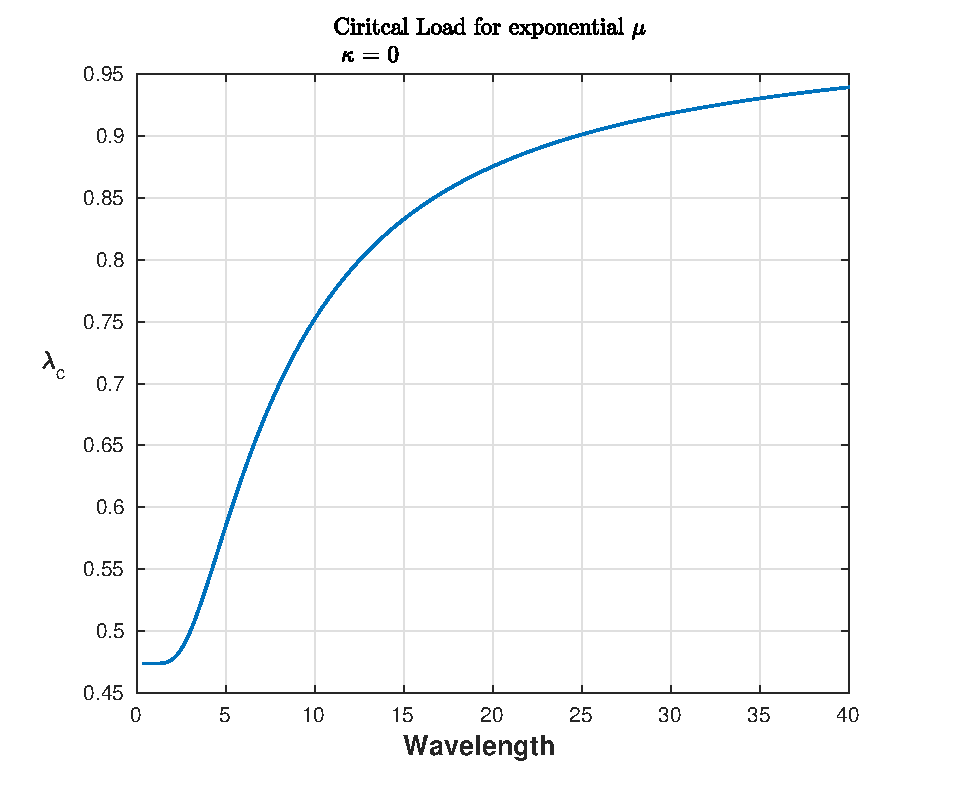
\includegraphics[width=\textwidth]{crit_load_kappa_0}
		\caption{$\kappa = 0$}
		\label{fig:crit_load_kappa_0}
	\end{subfigure}
	\begin{subfigure}[b]{0.33\textwidth}
		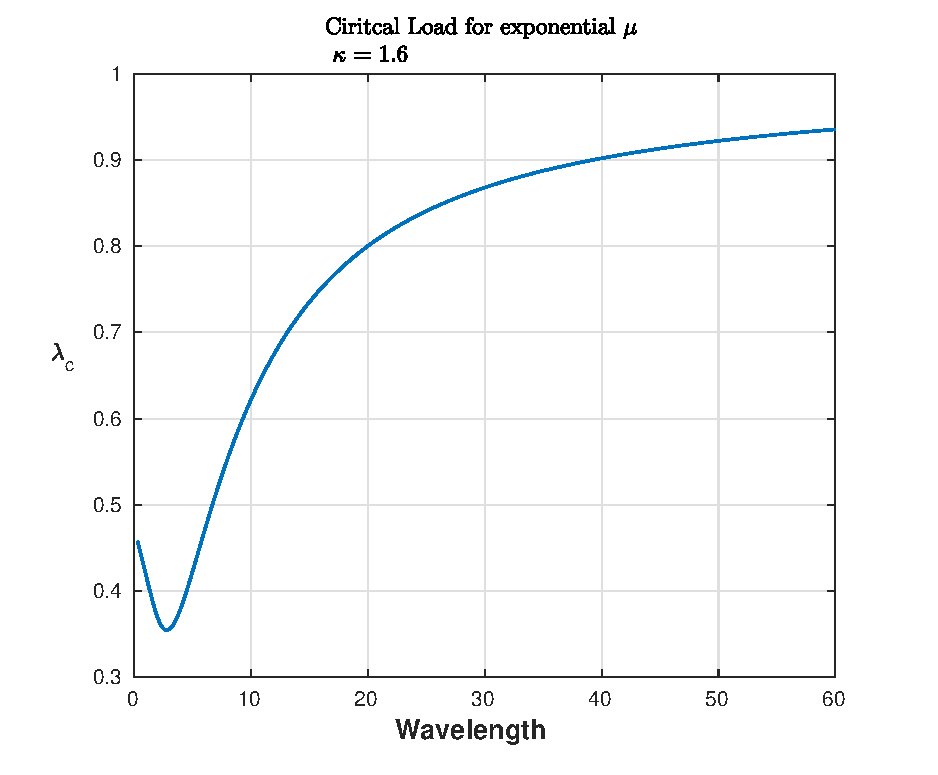
\includegraphics[width=\textwidth]{crit_load_kappa_1_6}
		\caption{$\kappa = 1.6$}
		\label{fig:crit_load_kappa_1_6}
	\end{subfigure}
	\begin{subfigure}[b]{0.33\textwidth}
		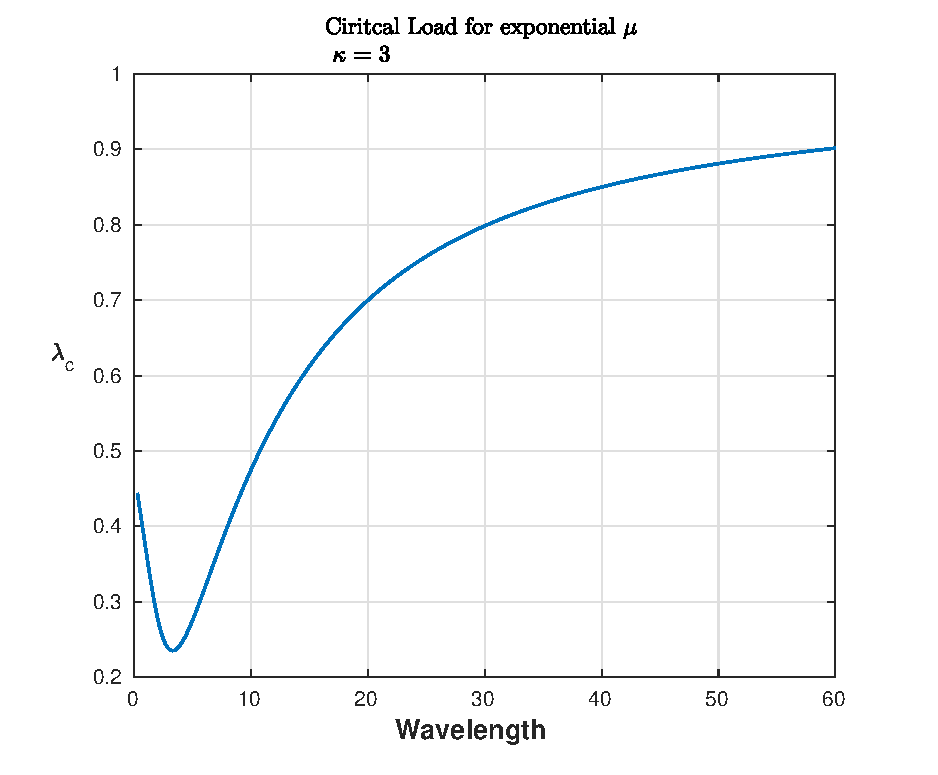
\includegraphics[width=\textwidth]{crit_load_kappa_3_0}
		\caption{$\kappa = 3.0$}
		\label{fig:crit_load_kappa_3_0}
	\end{subfigure}
	\caption{Critical loads for different wavelengths.}
    \label{fig:crit_load}
\end{figure}

\newpage
\section{Following the Bifurcated Solution}

	A finite element model was constructed as discussed in Appendix \ref{append_finite_element}. Primite cells were constructed with a lengths in the $x_1$ direction equal to the wavelength corresponding to the minimum critical loads as in Figures \ref{fig:crit_load_kappa_1_6} and \ref{fig:crit_load_kappa_3_0}. A bisection algorithm was employed to find the value of $\lambda$ when the principle solution becomes unstable (when the stiffness matrix loses positive-definiteness). Then, a pseduo-archlength algorithm was used to follow the unstable mode. Along this path, Bloch-wave eigenvalues were calculated. Thus, the stability of a path could be analyzed.


For $\kappa = 1.6$, the bifurcation diagram can be seen in Figure \ref{fig:bif_diagram_1_6_0} , plotting the loading parameter $\lambda$ with the congugate loading value $\Lambda= \frac{\partial \mathcal{E}}{\partial \lambda}$. A plot of $\lambda$ vs the L-2 norm of the displacements (relative to the principle solution) is also shwon for easier visualization. The Bloch-wave calculation showed that immediatly after initial bifurcation from the principle solution, there were unstable modes. The mode with wavelength equal to the primitivel cell length was also noted to be unstable. As the solution moved farther along this first bifurcated path, instabilities continued to emerge.
\begin{figure}[!htb]
	\begin{subfigure}[b]{0.5\textwidth}
		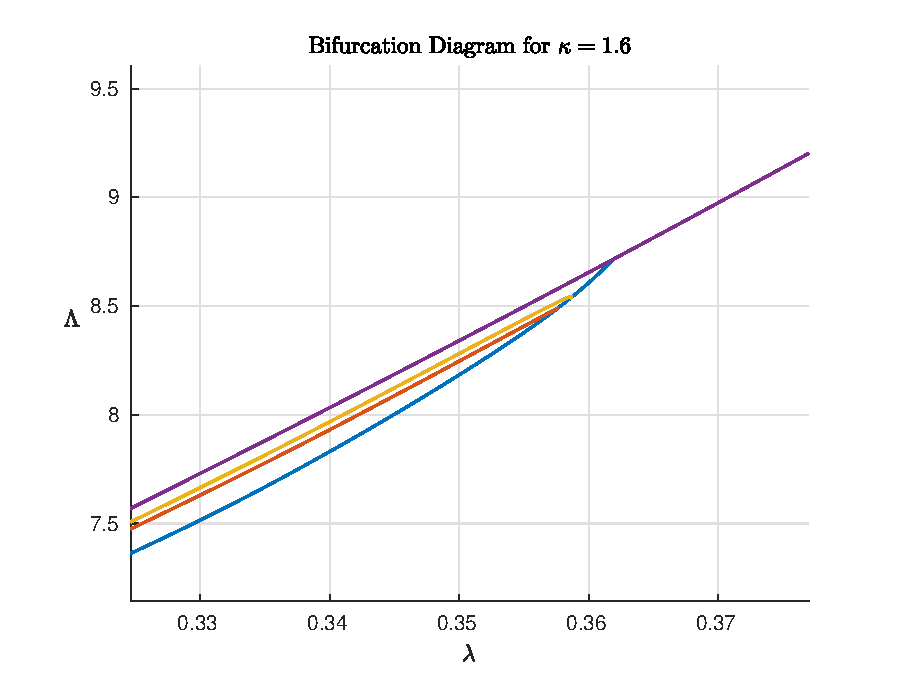
\includegraphics[width=\textwidth]{bif_diagram_1_6_0}
		\caption{$\lambda$ vs the conguate loading value $\Lambda = \frac{\partial \mathcal{E}}{\partial\lambda}$}
		\label{fig:bif_diagram_1_6_delta}
	\end{subfigure}
	\begin{subfigure}[b]{0.5\textwidth}
		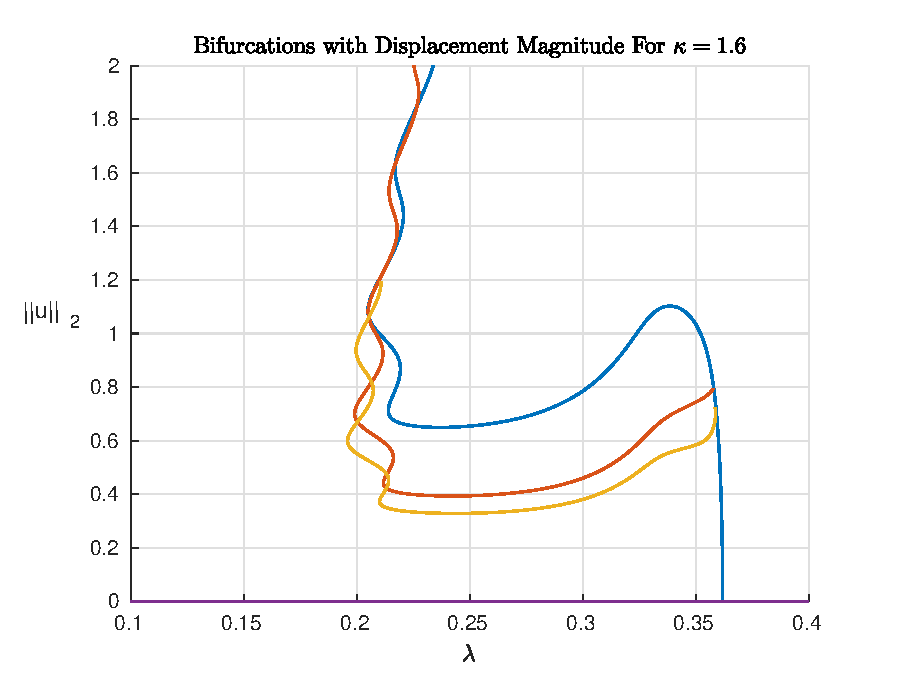
\includegraphics[width=\textwidth]{bif_diagram_disp_1_6_0}
		\caption{$\lambda$ vs L-2 norm of the displacements from the principle solution. }
		\label{fig:bif_diagram_1_6_disp}
	\end{subfigure}
	\captionsetup{format=hang}
	\caption{Bifurcation diagrams for the compressed strip with exponential $\mu$ and $\kappa = 1.6$. The purple curve is the principle solution. The blue, red, and yellow curves are the one, two, and three primitive cell paths, respectively.}
    \label{fig:bif_diagram_1_6_0}
\end{figure}
The deformations associated with various paths can be seen in Figures \ref{fig:mesh_1_6_1}, \ref{fig:mesh_1_6_2}, and \ref{fig:mesh_1_6_3}.
\begin{figure}[!htb]
	\begin{subfigure}[b]{0.33\textwidth}
		\includegraphics[width=\textwidth]{mesh/mesh_1_6_1_low}
	\end{subfigure}
	\begin{subfigure}[b]{0.33\textwidth}
		\includegraphics[width=\textwidth]{mesh/mesh_1_6_1_med}
	\end{subfigure}
    \begin{subfigure}[b]{0.33\textwidth}
		\includegraphics[width=\textwidth]{mesh/mesh_1_6_1_high}
	\end{subfigure}
	\captionsetup{format=hang}
	\caption{Deformed configurations of the single primitive cell with $\kappa = 1.6$ following the initial bifurcation. This is along the blue path in Figure \ref{fig:bif_diagram_1_6_0}.}
    \label{fig:mesh_1_6_1}
\end{figure}

\begin{figure}[!htb]
	\begin{subfigure}[b]{0.5\textwidth}
		\includegraphics[width=\textwidth]{mesh/mesh_1_6_2_low}
	\end{subfigure}
    \begin{subfigure}[b]{0.5\textwidth}
		\includegraphics[width=\textwidth]{mesh/mesh_1_6_2_high}
	\end{subfigure}
	\captionsetup{format=hang}
	\caption{Deformed configurations of the two primitive cell with $\kappa = 1.6$ following the initial bifurcation. This is along the red path in Figure \ref{fig:bif_diagram_1_6_0}. Much like the single primite cell case, the solution continues to a similar interpenetration at the localization in the middle.}
    \label{fig:mesh_1_6_2}
\end{figure}

\begin{figure}[!htb]
	\begin{subfigure}[b]{0.5\textwidth}
		\includegraphics[width=\textwidth]{mesh/mesh_1_6_3_low}
	\end{subfigure}
    \begin{subfigure}[b]{0.5\textwidth}
		\includegraphics[width=\textwidth]{mesh/mesh_1_6_3_high}
	\end{subfigure}
	\captionsetup{format=hang}
	\caption{Deformed configurations of the two primitive cell with $\kappa = 1.6$ following the initial bifurcation. This is along the yellow path in Figure \ref{fig:bif_diagram_1_6_0}. Much like the single primite cell case, the solution continues to a similar interpenetration at the localization in the middle.}
    \label{fig:mesh_1_6_3}
\end{figure}

\newpage
For $\kappa = 3.0$, the bifurcation diagram can be seen in Figure \ref{fig:bif_diagram_3_0}. Immediatly after initial bifurcation, the Bloch-wave caluclation showed that there were unstable modes. It was noted that the mode with wavelength equal to the primitive cell length was stable (differing from the $\mu = 1.6$ case).
The deformations associated with various paths can be seen in Figures \ref{fig:mesh_3_0_1}, \ref{fig:mesh_3_0_2}, and \ref{fig:mesh_3_0_3}.

\begin{figure}[!htb]
	\begin{center}
		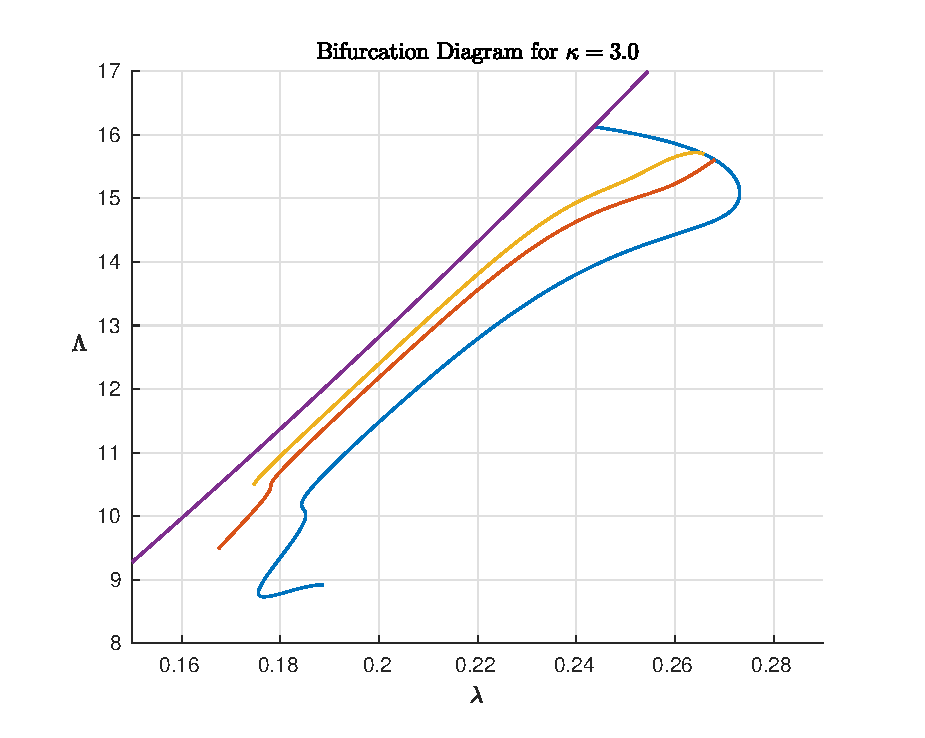
\includegraphics[scale=0.7]{bif_diagram_3_0}
	\end{center}
	\captionsetup{format=hang}
	\caption{Bifurcation diagram for the compressed strip with exponential $\mu$ and $\kappa = 3.0$. The purple curve is the principle solution. The blue, red, and yellow curves are the one, two, and three primitive cell paths, respectively.}
	\label{fig:bif_diagram_3_0}
\end{figure}

 \begin{figure}[!htb]
	\begin{subfigure}[b]{0.33\textwidth}
		\includegraphics[width=\textwidth]{mesh/mesh_3_0_1_low}
	\end{subfigure}
	\begin{subfigure}[b]{0.33\textwidth}
		\includegraphics[width=\textwidth]{mesh/mesh_3_0_1_med}
	\end{subfigure}
    \begin{subfigure}[b]{0.33\textwidth}
		\includegraphics[width=\textwidth]{mesh/mesh_3_0_1_high}
	\end{subfigure}
	\captionsetup{format=hang}
	\caption{Deformed configurations of the single primitive cell with $\kappa = 3.0$ following the initial bifurcation. This is along the blue path in Figure \ref{fig:bif_diagram_3_0}.}
    \label{fig:mesh_3_0_1}
\end{figure}

\begin{figure}[!htb]
	\begin{subfigure}[b]{0.5\textwidth}
		\includegraphics[width=\textwidth]{mesh/mesh_3_0_2_low}
	\end{subfigure}
    \begin{subfigure}[b]{0.5\textwidth}
		\includegraphics[width=\textwidth]{mesh/mesh_3_0_2_high}
	\end{subfigure}
	\captionsetup{format=hang}
	\caption{Deformed configurations of the two primitive cell with $\kappa = 3.0$ following the initial bifurcation. This is along the red path in Figure \ref{fig:bif_diagram_3_0}. Much like the single primite cell case, the solution continues to a similar interpenetration at the localization in the middle.}
    \label{fig:mesh_3_0_2}
\end{figure}

\begin{figure}[!htb]
	\begin{subfigure}[b]{0.5\textwidth}
		\includegraphics[width=\textwidth]{mesh/mesh_3_0_3_low}
	\end{subfigure}
    \begin{subfigure}[b]{0.5\textwidth}
		\includegraphics[width=\textwidth]{mesh/mesh_3_0_3_high}
	\end{subfigure}
	\captionsetup{format=hang}
	\caption{Deformed configurations of the two primitive cell with $\kappa = 3.0$ following the initial bifurcation. This is along the yellow path in Figure \ref{fig:bif_diagram_3_0}. Much like the single primite cell case, the solution continues to a similar interpenetration at the localization now on the edges.}
    \label{fig:mesh_3_0_3}
\end{figure}

A further study would investigate the larger values of $\kappa$. This would require an even finer mesh for the steep exponential.

\chapter{Piecewise Constant $\mu(x_2)$}
Next, a piecewise constant $\mu(x_2)$ function will be considered, of the form:
\begin{equation}
\mu(x_2) =
\left \{
\begin{aligned}
  \mu &= \mu_1 \qquad 0 \leq x_2 < L_1 \\
  \mu &= \mu_2 \qquad L_1 \leq x_2 \leq L_2
\end{aligned}
\right \}
\end{equation}
Thus, $\mu$ is constant in the differently shaded regions in Figure \ref{fig:stripFig_const}.
\begin{figure}[h]
	\begin{center}
		\includegraphics[scale=0.7]{compressed_strip_drawing_piece_const}
	\end{center}
	\captionsetup{format=hang}
	\caption{Diagram of the regions of piecewise constant $\mu$.}
	\label{fig:stripFig_const}
\end{figure}
\section{Initial Birfurcation}

Similarly to the other case, the PDE is separable, and results in a solution with two modes:

\begin{equation} \label{eq:piece_const_u1_modes}
\mathcal{A}^2 =
\left \{
\begin{aligned}
  \overset{1}{u}_1 &= -v_1(x_2)\sin(\omega x_1) \\
  \overset{1}{u}_2 &=  v_2(x_2)\cos(\omega x_1)
\end{aligned}
\right \} , \qquad
\mathcal{S}^2 =
\left \{
\begin{aligned}
  \overset{1}{u}_1 &= v_1(x_2)\cos(\omega x_1) - v_1(0) \\
  \overset{1}{u}_2 &=  v_2(x_2)\sin(\omega x_1)
\end{aligned}
\right \},
\end{equation}
Where the $x_1$ dependence above is identical to that of the exponential case. And the $x_2$ dependence is:
\begin{equation} \label{eq:piece_const_u1_v}
\begin{aligned}
v_1(x_2) &=
\left \{
\begin{aligned}
  \overset{1}{v}_1(x_2) &= \sum_{i = 1}^{4}A_ie^{\alpha_i x_2} \qquad 0 \leq x_2 < L_1 \\
  \overset{2}{v}_1(x_2) &= \sum_{i = 1}^{4}\bar{A}_ie^{\alpha_i x_2} \qquad L_1 \leq x_2 \leq L_2
\end{aligned}
\right \} \\
\\
v_2(x_2) &=
\left \{
\begin{aligned}
  \overset{1}{v}_2(x_2) &= \sum_{i = 1}^{4} A_i B_i e^{\alpha_i x_2} \qquad 0 \leq x_2 < L_1 \\
  \overset{2}{v}_2(x_2) &= \sum_{i = 1}^{4} \bar{A}_i B_i e^{\alpha_i x_2} \qquad L_1 \leq x_2 \leq L_2
\end{aligned}
\right \}.
\end{aligned}
\end{equation}
By a similar method to Appendix \ref{append_first_load}, this solution can be put into the boundry conditions for the domains of the piecewise solution. Then, for a given wavelength, the critical load can be solved for.

Using $\frac{L_1}{L_2} = 0.9$ and a ratio of $\frac{\mu_2}{\mu_1}$ of 10, the critical load was calculated for different wavelengths (Figure \ref{fig:piece_const_load}). There is a minimum $\lambda_c$ that occurrs at a unique wavelength.
\begin{figure}[!htb]
	\begin{center}
		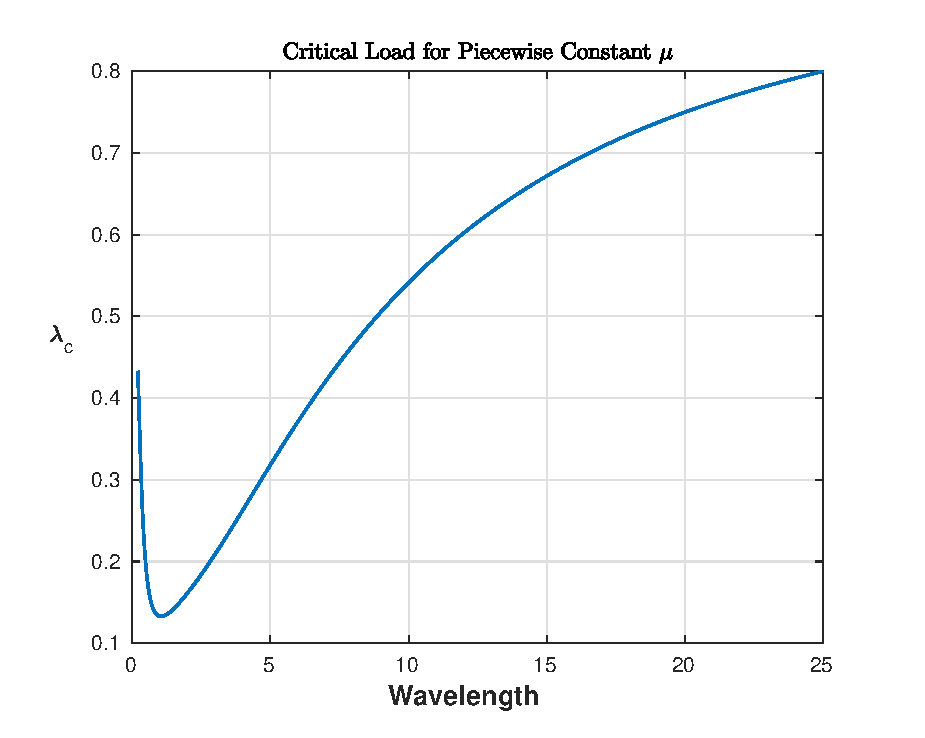
\includegraphics[scale=0.7]{crit_load_muRat_10}
	\end{center}
	\captionsetup{format=hang}
	\caption{Critical load for the first bifurcation using a piecewise constant $\mu$ using $\frac{L_1}{L_2} = 0.9$ and a ratio of $\frac{\mu_2}{\mu_1} = 10$.}
	\label{fig:piece_const_load}
\end{figure}

\newpage
\section{Following Bifurcated Solution}
A finite element model with length in the $x_1$ direction equal to the wavelength corresponding to the minimum $\lambda_c$ (from Figure \ref{fig:piece_const_load}) was constructed. A furthur discussion of the finer details can be found in Appendix \ref{append_finite_element}. The inital bifurcation was followed with a pseudo-archlength algorithim. Along this path, a Bloch-wave calculation gave eigenvalues for all modes. Upon initial bifurcation, the solution is stable for all modes. But furthur along this path, the double period mode goes unstable. This bifurcated path was also followed. A bifurcation diagram can be seen in Figure \ref{fig:piece_const_bif_diagram}.
\begin{figure}[!htb]
	\begin{center}
		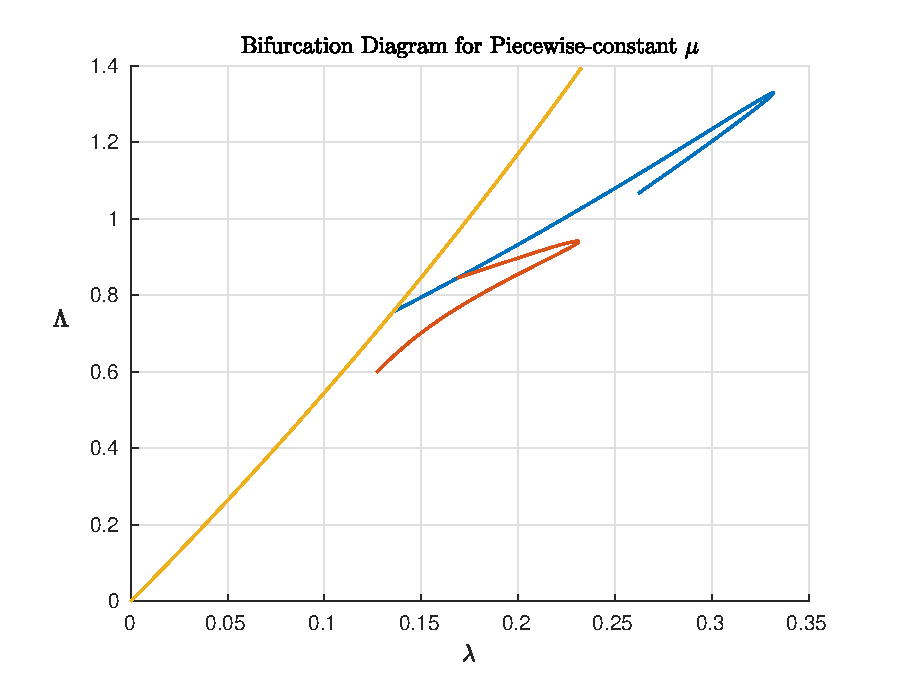
\includegraphics[scale=0.7]{bif_diagram_pieceConst_10_9}
	\end{center}
	\captionsetup{format=hang}
	\caption{Bifurcation diagram for the compressed strip with piecewise-constant $\mu$ using $\frac{L_1}{L_2} = 0.9$ and a ratio of $\frac{\mu_2}{\mu_1} = 10$. The yellow curve is the principle solution. The blue, and red curves are the one, and two primitive cell paths, respectively.}
	\label{fig:piece_const_bif_diagram}
\end{figure}

The deformations associated with these paths can be seen in Figures
\ref{fig:mesh_piece_const_10_9_1} and \ref{fig:mesh_piece_const_10_9_2}. A further study will analyze the stability of the two-period bifurcation (red curve in \ref{fig:piece_const_bif_diagram}).
\begin{figure}[!htb]
\begin{center}
	\begin{subfigure}[b]{0.22\textwidth}
		\includegraphics[width=\textwidth]{mesh/mesh_piece_const_10_9_1_low}
	\end{subfigure}
	\begin{subfigure}[b]{0.22\textwidth}
		\includegraphics[width=\textwidth]{mesh/mesh_piece_const_10_9_1_med}
	\end{subfigure}
    \begin{subfigure}[b]{0.22\textwidth}
		\includegraphics[width=\textwidth]{mesh/mesh_piece_const_10_9_1_high}
	\end{subfigure}
	\begin{subfigure}[b]{0.22\textwidth}
		\includegraphics[width=\textwidth]{mesh/mesh_piece_const_10_9_1_super}
	\end{subfigure}
\end{center}
	\captionsetup{format=hang}
	\caption{Deformed configurations following initial bifurcation of the single primitive cell with piecewise-constant $\mu$ using $\frac{L_1}{L_2} = 0.9$ and a ratio of $\frac{\mu_2}{\mu_1} = 10$. This is along the blue path in Figure \ref{fig:piece_const_bif_diagram}.}
    \label{fig:mesh_piece_const_10_9_1}
\end{figure}

\begin{figure}[!htb]
	\begin{subfigure}[b]{0.33\textwidth}
		\includegraphics[width=\textwidth]{mesh/mesh_piece_const_10_9_2_low}
	\end{subfigure}
	\begin{subfigure}[b]{0.33\textwidth}
		\includegraphics[width=\textwidth]{mesh/mesh_piece_const_10_9_2_med}
	\end{subfigure}
    \begin{subfigure}[b]{0.33\textwidth}
		\includegraphics[width=\textwidth]{mesh/mesh_piece_const_10_9_2_high}
	\end{subfigure}
	\captionsetup{format=hang}
	\caption{Deformed configurations following bifurcation of the two primitive cell with piecewise-constant $\mu$ using $\frac{L_1}{L_2} = 0.9$ and a ratio of $\frac{\mu_2}{\mu_1} = 10$. This is along the red path in Figure \ref{fig:piece_const_bif_diagram}.}
    \label{fig:mesh_piece_const_10_9_2}
\end{figure}


\begin{appendices}
  \chapter{Principle Solution Derivation} \label{append_principle}
For our principle solution, we will assume that $\overset{0}{\mathbf{F}}$ is constant throughout the domain and is of the form $\overset{0}{\mathbf{F}} = \diag[\lambda_1,\lambda_2]$. Then, the Priola-Kirchoff stress evaluated on this proposed solution in a orthonormal basis aligned with the $x_1$ and $x_2$ axis is:
\begin{equation} \label{eq:dW_dF_F0}
\left . \frac{\partial W}{\partial \mathbf{F}} \right|_{\overset{0}{\mathbf{F}}} = \diag[\Pi_{11}, \Pi_{22}],
\end{equation}
where $\Pi_{11}$ and $\Pi_{22}$ are defined are:
\begin{equation*}
\begin{aligned}
\Pi_{11} &= \mu(x_2) \left [ \lambda_1 - \lambda_1^{-1} + \frac{2\nu}{1 -\nu}(\lambda_1 \lambda_2^2 - \lambda_2) \right ] , \\
\Pi_{22} &= \mu(x_2) \left [ \lambda_2 - \lambda_2^{-1} + \frac{2\nu}{1 - \nu}(\lambda_1^2 \lambda_2 - \lambda_1) \right ].
\end{aligned}
\end{equation*}
Enforcing the zero normal traction on the free surface at $x_2 = L$ gives:
\begin{equation} \label{eq:lambda_relation}
\Pi_{22} |_{x_2 = L} = 0  \qquad \implies \qquad \lambda_2 - \lambda_2^{-1} + \frac{2\nu}{1 - \nu}(\lambda_1^2 \lambda_2 - \lambda_1) = 0.
\end{equation}
Thus, \eqref{eq:lambda_relation} gives a relationship for $\lambda_2$ in terms of $\lambda_2$ in the form of a quadratic. For equillibrium of this principle solution the following must be satisfied:
\begin{equation} \label{eq:eqbrm}
\mathcal{E},_{\mathbf{u}}\cdot \delta\mathbf{u} = \int_\Omega \left . \frac{\partial W}{\partial {F_{ij}}} \right |_{\overset{0}{\mathbf{F}}} \delta F_{ij} \,dA = 0.
\end{equation}
This can be shown to be true by noting that for the displacement control in the $x_1$ direction requires that $\int_{-\infty}^{\infty} \delta F_{11} \,dx_1 = 0$. Thus, the uniform stretching meets equilibrium criteria and passes through the origin. The stability can be shown from the positive definiteness of the incremental modulii for small $\lambda_1$. (I wil type this up later)

  \chapter{Initial Bifurcation Derivation} \label{append_first_sol}

The second variation of the energy is:
\begin{equation} \label{eq:second_var}
(\mathcal{E},_{\mathbf{u} \mathbf{u}}\cdot \delta\mathbf{u}) \cdot \delta\hat{\mathbf{u}} = \int_\Omega  \frac{\partial W}{\partial F_{ij} F_{kl}} \delta F_{ij} \delta \hat{F}_{kl} \,dA.
\end{equation}
The first bifurcated solution $\overset{1}{\mathbf{u}}$ occurs at a critical loading $\lambda_c$ when the following condition is met:
\begin{equation}
(\mathcal{E},_{\mathbf{u} \mathbf{u}}(\overset{0}{\mathbf{u}}, \lambda_c) \cdot \overset{1}{\mathbf{u}}) \cdot \delta\mathbf{u} = \int_\Omega  \left. \frac{\partial W}{\partial F_{ij} F_{kl}} \right |_{\lambda_c} \overset{1}{u}_{i,j} \delta u_{k,l} \,dA = 0,
\end{equation}
where the variations of deformation gradient have been replaced with equivalent variations of the displacement gradient. Integrating by parts and applying divergence theorem gives:
\begin{equation} \label{eq:byparts}
\int_{\partial \Omega} L^c_{ijkl}(x_2) \: \overset{1}{u}_{i,j} \: n_l \:  \delta u_k \: \,ds - \int_{\Omega} \left ( L^c_{ijkl}(x_2) \: \overset{1}{u}_{i,j} \right )_{,l} \: \delta u_k \: \,dA = 0,
\end{equation}
where $\left. \frac{\partial W}{\partial F_{ij} F_{kl}} \right |_{\lambda_c}$ has been replaced by $L^c_{ijkl}(x_2)$ for brevity, and $n_{i}$ is the unit normal of $\partial \Omega$. 

\section{Exponential}
The surface integral in \eqref{eq:byparts} the natural boundary conditions. The boundary conditions on the free surface at $x_2 = L$ are:
\begin{equation} \label{eq:bcAtL}
\left . L^c_{ij12} \: \overset{1}{u}_{i,j} \right |_{x_2 = L} = 0, \qquad
\left . L^c_{ij22} \: \overset{1}{u}_{i,j} \right |_{x_2 = L} = 0,
\end{equation}
which correspond to the absence of shear and normal traction, respectfully. The natural boundary condition at $x_2 = 0$ is:
\begin{equation} \label{eq:shearAt0}
\left . L^c_{ij12}(0) \: \overset{1}{u}_{i, j}  \right |_{x_2 = 0} = 0,
\end{equation}
which corresponds to no shear tractions at $x_2 = 0$. There is also the condition that the $x_2$ displacement at $x_2 = 0$ is fixed:
\begin{equation} \label{eq:dispAt0}
\left . u_2 \right |_{x_2 = 0} = 0 .
\end{equation}
The integrand over the domain in \eqref{eq:byparts} gives a system of two linear PDE's:
\begin{equation}
\begin{aligned}
L^c_{ij12,2} \: \overset{1}{u}_{i,j} + L^c_{ij1l} \: \overset{1}{u}_{i,jl} &= 0, \\
L^c_{ij22,2} \: \overset{1}{u}_{i,j} + L^c_{ij2l} \: \overset{1}{u}_{i,jl} &= 0 ,
\end{aligned}
\end{equation}
where the incremental moduli's exclusive dependent on $x_2$ has been used to simplify the expression. This system of PDE's can then be expanded, using the symmetry of the incremental moduli to simplify the expression, giving:
\begin{equation} \label{eq:rawpde}
\begin{aligned}
L^c_{2112,2} \: \overset{1}{u}_{2,1} + L^c_{1212,2} \: \overset{1}{u}_{1,2} + L^c_{1111} \: \overset{1}{u}_{1,11} + L^c_{1212} \: \overset{1}{u}_{1,22}+ L^c_{2112} \: \overset{1}{u}_{2,12}  + L^c_{1122} \: \overset{1}{u}_{2,21} &= 0, \\
L^c_{1122,2} \: \overset{1}{u}_{1,1} + L^c_{2222,2} \: \overset{1}{u}_{2,2} + L^c_{2222} \: \overset{1}{u}_{2,22}+ L^c_{1212} \: \overset{1}{u}_{2,11}+ L^c_{2112} \: \overset{1}{u}_{1,12}  + L^c_{2211} \: \overset{1}{u}_{1,21} &= 0.
\end{aligned}
\end{equation}
The form of the parameter $\mu(x_2)$ will now be introduced. It will be chosen to be an exponential of the form:
\begin{equation}
\mu(x_2) = \mu_0 e^{\kappa x_2}.
\end{equation}
Then, it can be seen that all of the $L^c_{ijkl}$'s are simply constant values multiplied with $\mu(x_2)$. Then with the chosen form of $\mu$, $L^c_{ijkl,2} = \kappa L^c_{ijkl}$. Applying this to \eqref{eq:rawpde} gives:
\begin{equation} \label{eq:pde}
\begin{aligned}
\kappa \tilde{L}^{c}_{2112} \: \overset{1}{u}_{2,1} + \kappa \tilde{L}^{c}_{1212} \: \overset{1}{u}_{1,2} + \tilde{L}^{c}_{1111} \: \overset{1}{u}_{1,11} + \tilde{L}^{c}_{1212} \: \overset{1}{u}_{1,22}+ \tilde{L}^{c}_{2112} \: \overset{1}{u}_{2,12}  + \tilde{L}^{c}_{1122} \: \overset{1}{u}_{2,21} &= 0,\\
\kappa \tilde{L}^{c}_{1122} \: \overset{1}{u}_{1,1} + \kappa \tilde{L}^{c}_{2222} \: \overset{1}{u}_{2,2} + \tilde{L}^{c}_{2222} \: \overset{1}{u}_{2,22}+ \tilde{L}^{c}_{1212} \: \overset{1}{u}_{2,11}+ \tilde{L}^{c}_{2112} \: \overset{1}{u}_{1,12}  + \tilde{L}^{c}_{2211} \: \overset{1}{u}_{1,21} &= 0,
\end{aligned}
\end{equation}
where $\tilde{L}^{c}_{ijkl}$ is the constant part of $L^{c}_{ijkl}$ (${L}^{c}_{ijkl} = \mu(x_2) \tilde{L}^{c}_{ijkl}$), as both equations have been divided throughout by $\mu(x_2)$.
This system of linear PDE's with constant coefficients can be separated (I will type this up later), admitting the following form of the solution:
\begin{equation} \label{eq:u1_vals}
\mathcal{A}^2 :
\left \{
\begin{aligned}
  \overset{1}{u}_1 &= -v_1(x_2)\sin(\omega x_1) \\
  \overset{1}{u}_2 &=  v_2(x_2)\cos(\omega x_1)
\end{aligned}
\right \} , \qquad
\mathcal{S}^2 :
\left \{
\begin{aligned}
  \overset{1}{u}_1 &= v_1(x_2)\cos(\omega x_1) - v_1(0) \\
  \overset{1}{u}_2 &=  v_2(x_2)\sin(\omega x_1)
\end{aligned}
\right \},
\end{equation}
where $\mathcal{A}^2$ and $\mathcal{S}^2$ denote the symmetric and antisymmetric $u_1$ modes about the $x_2$ axis, respectfully. $\omega$ is an arbitrary constant that arises from the separation of the system of linear PDE's, and is realted to the wavelength of the instable mode. The $x_2$ dependence is:
\begin{equation} \label{eq:exp_u1_v}
v_1(x_2) = \sum_{i = 1}^{4}A_ie^{\alpha_i x_2}, \qquad v_2(x_2) = \sum_{i = 1}^{4} A_i B_i e^{\alpha_i x_2}.
\end{equation}
These solutions can be substituted into the original system of PDE's in \eqref{eq:pde}. This results in the $\alpha_i$'s being the roots to the following quartic characteristic equation:
\begin{equation} \label{eq:characteristic}
a\alpha^4 + b\alpha^3 + c\alpha^2 + d\alpha + e = 0,
\end{equation}
where the coefficients are:
\begin{equation*}
\begin{aligned}
  a &= \tilde{L}^{c}_{2222}\tilde{L}^{c}_{1212}, \\
  b &= 2\kappa \tilde{L}^{c}_{2222}\tilde{L}^{c}_{1212}, \\
  c &= \omega^2 \left[ \left ( \tilde{L}^{c}_{1122} + \tilde{L}^{c}_{2112}\right )^2 - \left ( \tilde{L}^{c}_{1212} \right )^2 - \tilde{L}^{c}_{1111}\tilde{L}^{c}_{2222} + \frac{\kappa^2}{\omega^2}\tilde{L}^{c}_{2222}\tilde{L}^{c}_{1212}    \right ], \\
  d &= \kappa \omega^2 \left[ \left ( \tilde{L}^{c}_{1122} + \tilde{L}^{c}_{2112}\right )^2 - \left ( \tilde{L}^{c}_{1212} \right )^2 - \tilde{L}^{c}_{1111}\tilde{L}^{c}_{2222} \right ], \\
  e &= \omega^2 \left( \kappa^2 \tilde{L}^{c}_{1122}\tilde{L}^{c}_{2112} + \omega^2 \tilde{L}^{c}_{1111}\tilde{L}^{c}_{1212}. \right)
\end{aligned}
\end{equation*}
Substituiting the form of the solution into the original system also gives the relationship for the coefficents $B_i$'s:
\begin{equation}
B_i = \frac {\omega^2 \tilde{L}^{c}_{1111} - \kappa \tilde{L}^{c}_{1212} \alpha_i - \tilde{L}^{c}_{1212} \alpha_i^2 }
            {\omega \left (\tilde{L}^{c}_{2112} + \tilde{L}^{c}_{1122} \right) \alpha_i + \omega \kappa \tilde{L}^{c}_{2112}}
\end{equation}
Now the solution will be substituted into the four boundary conditions. The shear traction condition at $x_2 = L$ in \eqref{eq:bcAtL}  requires:
\begin{equation}
\sum_{i = 1}^4 \left[ \omega \tilde{L}^{c}_{2112} A_iB_i e^{\alpha_iL} + \tilde{L}^{c}_{1212} \alpha_i A_i e^{\alpha_i L} \right ] = 0.
\end{equation}
The normal traction condition at $x_2 = L$ in \eqref{eq:bcAtL}  requires:
\begin{equation}
\sum_{i = 1}^4 \left [ \tilde{L}^{c}_{2222} \alpha_i A_i B_i e^{\alpha_i L} - \omega \tilde{L}^{c}_{1122} A_i e^{\alpha_i L} \right ] = 0 .
\end{equation}
The shear traction condition at $x_2 = 0$ in \eqref{eq:shearAt0} requires:
\begin{equation}
\sum_{i = 1}^4 \left [ \tilde{L}^{c}_{1212} \alpha_iA_i + \omega \tilde{L}^{c}_{2112} A_i B_i \right ] = 0.
\end{equation}
And lastly, the constrained vertical displacements at $x_2 = 0$ in equation \eqref{eq:dispAt0} requires:
\begin{equation}
\sum_{i=1}^4 A_i B_i = 0.
\end{equation}
These four boundary condition equations give four homogeneous equations for the four unknown $A_i$'s. These can be collected and put into matrix form:
\begin{equation}
\mathbf{M} \mathbf{A} = \mathbf{0},
\end{equation}
where $\mathbf{A}$ is the vector of amplitude $A_i$'s:
\begin{equation}
\mathbf{A} = [ A_1, A_2, A_3, A_4 ]^T.
\end{equation}
And $\mathbf{M}$ is the assembled matrix of coefficients from the boundary condition requirements. Then our first bifurcated solution occurs at the smallest $\lambda$ that satisfies:
\begin{equation} \label{eq:detM}
\mathrm{det}(\mathbf{M}) = 0.
\end{equation}
Then a procedure to find the critical load for a given wavelength mode would be to first evaluate the $\omega$ value for that mode, use that value to asseble the matrix $\mathbf{M}(\lambda)$, and then solve numerically for the lowest $\lambda > 0$ that satisfies \eqref{eq:detM}.

\section{Piecewise Constant}
Consider $\overset{1}{u}(x_1, x_2)$ of the form,
\begin{equation}
\overset{1}{u}(x_1, x_2) = \left \{ 
\begin{aligned}
\overset{1_1}{u}(x_1, x_2),  \quad 0 \leq x_2 < L_1,  \\
\overset{1_2}{u}(x_1, x_2),  \quad L_1 \leq x_2 \leq L_2
\end{aligned}
\right. 
\end{equation}
The integrals in \eqref{eq:byparts} can be broken into integrals over regions of constant $\mu$ giving,
\begin{equation} \label{eq:piece_const_weak}
\begin{gathered}
0 = \mu_1 \int_{\partial \Omega_1} \tilde{L}^c_{ijkl} \: \overset{1_1}{u}_{i,j} \: n_l \:  \delta u_k \: \,ds +  \mu_2 \int_{\partial \Omega_2} \tilde{L}^c_{ijkl} \: \overset{1_2}{u}_{i,j} \: n_l \:  \delta u_k \: \,ds \\
- \mu_1 \int_{\Omega_1} \tilde{L}^c_{ijkl} \: \overset{1_1}{u}_{i,jl} \: \delta u_k \: \,dA - \mu_2 \int_{\Omega_2}  \tilde{L}^c_{ijkl} \: \overset{1_2}{u}_{i,jl} \: \delta u_k \: \,dA
\end{gathered}
\end{equation}
Where,
\begin{equation}
L^c_{ijkl}(x_1, x_2) =
\left \{
\begin{aligned}
  \mu_1 \tilde{L}^c_{ijkl} , \quad  0 &\leq x_2 < L_1 \\
  \mu_2 \tilde{L}^c_{ijkl} , \quad  L_1 &\leq x_2 \leq L_2\\
\end{aligned}
\right.
\end{equation}
Then the area integrals of \eqref{eq:piece_const_weak} give the system of PDE's,
\begin{equation} \label{eq:piece_const_PDE_system}
\begin{aligned}
 \tilde{L}^{c}_{1111} \: \overset{1_{1,2}}{u}_{1,11} + \tilde{L}^{c}_{1212} \: \overset{1_{1,2}}{u}_{1,22}+ \tilde{L}^{c}_{2112} \: \overset{1_{1,2}}{u}_{2,12}  + \tilde{L}^{c}_{1122} \: \overset{1_{1,2}}{u}_{2,21} &= 0,\\
 \tilde{L}^{c}_{2222} \: \overset{1_{1,2}}{u}_{2,22}+ \tilde{L}^{c}_{1212} \: \overset{1_{1,2}}{u}_{2,11}+ \tilde{L}^{c}_{2112} \: \overset{1_{1,2}}{u}_{1,12}  + \tilde{L}^{c}_{2211} \: \overset{1_{1,2}}{u}_{1,21} &= 0,
\end{aligned}
\end{equation}
And the boundary integrals of \eqref{eq:piece_const_weak} give the boundary conditions,
\begin{equation} \label{eq:piece_const_u1_bcs}
\begin{aligned}
\overset{1_1}{u}_2(x_1, 0) &= 0 \\
\tilde{L}^c_{12kl} \: \overset{1_1}{u}_{k,l}(x_1, 0) &= 0 \\
\tilde{L}^c_{12kl} \: \overset{1_1}{u}_{k,l}(x_1, L_2) &= 0 \\
\tilde{L}^c_{22kl} \: \overset{1_2}{u}_{k,l}(x_1, L_2) &= 0 \\
\overset{1_1}{u}_1(x_1, L_1) - \overset{1_2}{u}_1(x_1, L_1) &= 0 \\
\overset{1_1}{u}_2(x_1, L_1) - \overset{1_2}{u}_2(x_1, L_1) &= 0 \\
\left ( \tilde{L}^c_{12kl} \: \overset{1_1}{u}_{k,l}(x_1, L_1) \right ) - \frac{\mu_2}{\mu_1} \left( \tilde{L}^c_{12kl} \: \overset{1_2}{u}_{k,l}(x_1, L_1) \right )  &= 0 \\
\left ( \tilde{L}^c_{22kl} \: \overset{1_1}{u}_{k,l}(x_1, L_1) \right ) - \frac{\mu_2}{\mu_1} \left( \tilde{L}^c_{22kl} \: \overset{1_2}{u}_{k,l}(x_1, L_1) \right )  &= 0
\end{aligned}
\end{equation}
The system of PDE's in \eqref{eq:piece_const_PDE_system} can be separated, admitting the following form of the solution:
\begin{equation} \label{eq:piece_const_u2_form}
\begin{aligned}
\mathcal{A}^2 : \left \{
\begin{aligned}
\overset{1}{u}_1(x_1, x_2) &= \left \{
\begin{aligned}
  \overset{1_1}{u}_1 &= -\overset{1}{v}_1(x_2) \sin( \omega x_1), \quad  0 \leq x_2 < L_1\\
  \overset{1_2}{u}_1 &= -\overset{2}{v}_1(x_2) \sin( \omega x_1), \quad  L_1 \leq x_2 \leq L_2 \\
\end{aligned}
\right.
\\
\overset{1}{u}_2(x_1, x_2) &= \left \{
\begin{aligned}
  \overset{1_1}{u}_2 &= \overset{1}{v}_2(x_2) \cos( \omega x_1), \quad  0 \leq x_2 < L_1\\
\overset{1_2}{u}_2 &= \overset{2}{v}_2(x_2) \cos( \omega x_1), \quad  L_1 \leq x_2 \leq L_2\\
\end{aligned}
\right.
\end{aligned}
\right \} \\
\\
\mathcal{S}^2 : \left \{
\begin{aligned}
\overset{1}{u}_1(x_1, x_2) &= \left \{
\begin{aligned}
  \overset{1_1}{u}_1 &= \overset{1}{v}_1(x_2) \cos(\omega x_1) - \overset{1}{v}_1(0), \quad  0 \leq x_2 < L_1\\
  \overset{1_2}{u}_1 &= \overset{2}{v}_1(x_2) \cos(\omega x_1) - \overset{1}{v}_1(0), \quad  L_1 \leq x_2 \leq L_2 \\
\end{aligned}
\right.
\\
\overset{1}{u}_2(x_1, x_2) &= \left \{
\begin{aligned}
  \overset{1_1}{u}_2 &= \overset{1}{v}_2(x_2) \sin(\omega x_1), \quad  0 \leq x_2 < L_1\\
\overset{1_2}{u}_2 &= \overset{2}{v}_2(x_2) \sin( \omega x_1), \quad  L_1 \leq x_2 \leq L_2\\
\end{aligned}
\right.
\end{aligned}
\right \}
\end{aligned}
\end{equation}
where $\mathcal{A}^2$ and $\mathcal{S}^2$ denote the symmetric and antisymmetric $u_1$ modes about the $x_2$ axis, respectfully. $\omega$ is an arbitrary constant that arises from the separation of the system of linear PDE's, and is realted to the wavelength of the instable mode. The $x_2$ dependence is:
\begin{equation} \label{eq:piece_const_u1_v}
\begin{aligned}
\overset{1}{v}_1(x_2) = \sum_{i = 1}^{4}A_ie^{\alpha_i x_2}, \qquad \overset{1}{v}_2(x_2) = \sum_{i = 1}^{4} A_i B_i e^{\alpha_i x_2} \\
\overset{2}{v}_1(x_2) = \sum_{i = 1}^{4}A_{i+4} e^{\alpha_i x_2}, \qquad \overset{2}{v}_2(x_2) = \sum_{i = 1}^{4} A_{i+4} B_i e^{\alpha_i x_2}
\end{aligned}
\end{equation}
These solutions can be substituted into the original system of PDE's in \eqref{eq:piece_const_PDE_system}. This results in the $\alpha_i$'s being the roots to the following quartic characteristic equation:
\begin{equation} \label{eq:piece_const_characteristic}
a\alpha^4 + c\alpha^2 + e = 0,
\end{equation}
with coefficents:
\begin{equation*}
\begin{aligned}
  a &= \tilde{L}^{c}_{2222}\tilde{L}^{c}_{1212}, \\
  c &= \omega^2 \left[ \left ( \tilde{L}^{c}_{1122} + \tilde{L}^{c}_{2112}\right )^2 - \left ( \tilde{L}^{c}_{1212} \right )^2 - \tilde{L}^{c}_{1111}\tilde{L}^{c}_{2222} + \frac{\kappa^2}{\omega^2}\tilde{L}^{c}_{2222}\tilde{L}^{c}_{1212}    \right ], \\
  e &= \omega^2 \left( \kappa^2 \tilde{L}^{c}_{1122}\tilde{L}^{c}_{2112} + \omega^2 \tilde{L}^{c}_{1111}\tilde{L}^{c}_{1212}. \right)
\end{aligned}
\end{equation*}
Substituiting the form of the solution into the original system also gives the relationship for the coefficents $B_i$'s:
\begin{equation}
B_i = \frac {\omega^2 \tilde{L}^{c}_{1111}  - \tilde{L}^{c}_{1212} \alpha_i^2 }
            {\omega \left (\tilde{L}^{c}_{2112} + \tilde{L}^{c}_{1122} \right) \alpha_i}
\end{equation}
Now the solution will be substituted into the eight boundary conditions of \eqref{eq:piece_const_u1_bcs}. This gives eight linear homogenous equations for the unknown coefficents $A_i$'s,
\begin{equation}
\begin{aligned}
\sum_{i=1}^4 A_i B_i &= 0 \\
\sum_{i=1}^4 \left[ \tilde{L}^c_{1212} \alpha_i A_i + \omega \tilde{L}^c_{2112} A_i B_i \right] &= 0 \\
\sum_{i=1}^4 \left[ \tilde{L}^c_{1212} \alpha_i A_{i+4} + \omega \tilde{L}^c_{2112} A_{i+4} B_i \right] e^{\alpha_i L_2} &= 0 \\
\sum_{i=1}^4 \left[ \tilde{L}^c_{2222} \alpha_i A_{i+4} B_i - \omega \tilde{L}^c_{1122} A_{i+4} \right] e^{\alpha_i L_2} &= 0 \\
\sum_{i=1}^4 A_i e^{\alpha_i L_1} - \sum_{i=1}^4 A_{i+4}e^{\alpha_i L_1} &= 0 \\
\sum_{i=1}^4 A_i B_i e^{\alpha_i L_1} - \sum_{i=1}^4 A_{i+4} B_i e^{\alpha_i L_1} &= 0 \\
\sum_{i=1}^4 \left[ \tilde{L}^c_{1212} \alpha_i A_{i} + \omega \tilde{L}^c_{2112} A_{i} B_i \right] e^{\alpha_i L_1} - \frac{\mu_2}{\mu_1}\sum_{i=1}^4 \left[ \tilde{L}^c_{1212} \alpha_i A_{i+4} + \omega \tilde{L}^c_{2112} A_{i+4} B_i \right] e^{\alpha_i L_1} &= 0 \\
\sum_{i=1}^4 \left[ \tilde{L}^c_{2222} \alpha_i A_{i} B_i - \omega \tilde{L}^c_{1122} A_{i} \right] e^{\alpha_i L_1} - \frac{\mu_2}{\mu_1} \sum_{i=1}^4 \left[ \tilde{L}^c_{2222} \alpha_i A_{i+4} B_i - \omega \tilde{L}^c_{1122} A_{i+4} \right] e^{\alpha_i L_1} &= 0
\end{aligned}
\end{equation}
These eight boundary condition equations give linear homogeneous equations for the unknown $A_i$'s. These can be collected and put into matrix form:
\begin{equation}
\mathbf{M} \mathbf{A} = \mathbf{0},
\end{equation}
where $\mathbf{A}$ is the vector of amplitude $A_i$'s:
\begin{equation}
\mathbf{A} = [ A_1, A_2, A_3, A_4, A_5, A_6, A_7, A_8 ]^T.
\end{equation}
And $\mathbf{M}$ is the assembled matrix of coefficients from the boundary condition requirements. Then our first bifurcated solution occurs at the smallest $\lambda$ that satisfies:
\begin{equation} \label{eq:detM}
\mathrm{det}(\mathbf{M}) = 0.
\end{equation}
Then a procedure to find the critical load for a given wavelength mode would be to first evaluate the $\omega$ value for that mode, use that value to asseble the matrix $\mathbf{M}(\lambda)$, and then solve numerically for the lowest $\lambda > 0$ that satisfies \eqref{eq:detM}.

  \chapter{Asymptotics} \label{asymp}
  The displacements, loading parameter, and congugate loading parameter will be expanded about the critical point with respect to th e bifurcation amplitutde parameter $\xi$, which is defined as,
  \begin{equation}
  \xi \equiv <\mathbf{u} - \overset{0}{\mathbf{u}}, \overset{1}{\mathbf{u}}>
  \end{equation}
  Where the inner product chosen for some fields $\mathbf{a}$ and $\mathbf{b}$ is,
  \begin{equation}
  <\mathbf{a}, \mathbf{b}> \equiv \frac{1}{|\Omega|} \int_\Omega \mathbf{a} \cdot \mathbf{b} \: dA
  \end{equation}
  Where $\Omega$ is the reference unit cell, and $|\Omega|$ is its area.
  
  The LSK expansion about the critical point for the symmetric bifurcation is then,
  \begin{equation}
  	\mathbf{u} = \overset{0}{\mathbf{u}}(\lambda) + \xi \overset{1}{\mathbf{u}} + \frac{\xi^2}{2} \overset{2}{\mathbf{u}} + \mathcal{O}(\xi^3) \:, \qquad \lambda = \lambda_c + \frac{\xi^2}{2} \lambda_2 + \mathcal{O}(\xi^4)
  \end{equation}
The conguate loading parameter $\Lambda$, defined by $\Lambda \equiv \frac{d \mathcal{E}}{d \lambda}$, can also be expanded as,
\begin{equation}
	\Lambda = \Lambda_c + \frac{\xi^2}{2} \Lambda_2 + \mathcal{O}(\xi^4)
\end{equation}
The coefficients from the expansion for $\mathbf{u}$ and $\lambda$ can be found as unique solutions to,
\begin{align}
(\mathcal{E}^c,_{\mathbf{u} \mathbf{u}} \overset{2}{\mathbf{u}} + (\mathcal{E}^c_{\mathbf{u} \mathbf{u} \mathbf{u}} \overset{1}{\mathbf{u}}) \overset{1}{\mathbf{u}} ) \delta \mathbf{v} = 0, \quad <\overset{1}{\mathbf{u}}, \delta\mathbf{v}> = 0   \label{eq:u2_eq}\\
\lambda_2 = -\frac{1}{3} \frac{(((\mathcal{E}^c_{\mathbf{u} \mathbf{u} \mathbf{u} \mathbf{u}} \overset{1}{\mathbf{u}}) \overset{1}{\mathbf{u}}) \overset{1}{\mathbf{u}}) \overset{1}{\mathbf{u}} 
		+ 3 ((\mathcal{E}^c,_{\mathbf{u} \mathbf{u} \mathbf{u}}\overset{2}{\mathbf{u}})\overset{1}{\mathbf{u}})\overset{1}{\mathbf{u}}}{((d\mathcal{E}^c,_{\mathbf{u} \mathbf{u}}/d\lambda)\overset{1}{\mathbf{u}})\overset{1}{\mathbf{u}}}
\end{align}
The coefficent for the expansion for $\Lambda$ can be found by taking two derivatives of the definition of $\Lambda$ with respect to $\xi$,
\begin{equation}
	\Lambda_2 =  ((d\mathcal{E}^c,_{\mathbf{u} \mathbf{u}}/d\lambda)\overset{1}{\mathbf{u}})\overset{1}{\mathbf{u}} + (d\mathcal{E}^c,_{\mathbf{u}}/d\lambda) \overset{2}{\mathbf{u}} + \lambda_2(d\mathcal{E}^c,_{\mathbf{u}}/d\lambda) \frac{d \overset{0}{\mathbf{u}}}{d \lambda}
\end{equation}

\section{Expoential Case}
To obtain $\lambda_2$ and $\Lambda_2$ and thus have stability information, $\overset{2}{\mathbf{u}}(x_1, x_2)$ will first need to be solved for from \eqref{eq:u2_eq},
\begin{equation} \label{eq:u2_eq_1}
\int_\Omega ( L^c_{ijkl}(x_2) \: \overset{2}{u}_{k,l} + M^c_{ijklmn}(x_2) \: \overset{1}{u}_{k,l} \: \overset{1}{u}_{m,n} ) \: \delta v_{i,j} \: dA = 0,  \quad <\overset{1}{\mathbf{u}}, \mathbf{v} > = 0
\end{equation} 
where,
\begin{equation*}
L^c_{ijkl}(x_2) = \frac{\partial^2 W(\overset{0}{\mathbf{u}}(\lambda_c))}{\partial F_{ij} \partial F_{kl}}, \qquad M^c_{ijklmn}(x_2) = \frac{\partial^3 W(\overset{0}{\mathbf{u}}(\lambda_c))}{\partial F_{ij} \partial F_{kl} \partial F_{mn}}
\end{equation*}
Integrating \eqref{eq:u2_eq_1} by parts and applying divergence theorem gives the weak form,
\begin{equation} \label{eq:exp_asy_weak}
\begin{split}
0 = \int_{\partial \Omega} \left( L^c_{ijkl}(x_2) \: \overset{2}{u}_{k,l} + M^c_{ijklmn}(x_2) \: \overset{1}{u}_{k,l} \: \overset{1}{u}_{m,n} \right) n_j \delta v_i ds \\ - \int_\Omega \left( L^c_{ijkl}(x_2) \: \overset{2}{u}_{k,l} + M^c_{ijklmn}(x_2) \: \overset{1}{u}_{k,l} \: \overset{1}{u}_{m,n} \right)_{,j} \delta v_i dA
\end{split}
\end{equation}
The first and second integrals in \eqref{eq:exp_asy_weak} gives the boundary conditions and system of linear PDE's for $\overset{2}{\mathbf{u}}$, respectfully. Thus, our system of linear PDE's are,
\begin{equation}
\left( L^c_{ijkl}(x_2) \: \overset{2}{u}_{k,l} \right)_{,j} = -\left( M^c_{ijklmn}(x_2) \: \overset{1}{u}_{k,l} \: \overset{1}{u}_{m,n} \right)_{,j} \qquad i = 1,2
\end{equation} 
Which can be expanded to,
\begin{align}
\begin{split}
\kappa \tilde{L}^{c}_{2112} \: \overset{2}{u}_{2,1} + \kappa \tilde{L}^{c}_{1212} \: \overset{2}{u}_{1,2} + \tilde{L}^{c}_{1111} \: \overset{2}{u}_{1,11} + \tilde{L}^{c}_{1212} \: \overset{2}{u}_{1,22}+ \tilde{L}^{c}_{2112} \: \overset{2}{u}_{2,12}  + \tilde{L}^{c}_{1122} \: \overset{2}{u}_{2,21} =  \\
-\left(\tilde{M}^c_{11kjmn}(\overset{1}{u}_{k,l} \: \overset{1}{u}_{m,n})_{,1} + \tilde{M}^c_{12kjmn}(\overset{1}{u}_{k,l} \: \overset{1}{u}_{m,n})_{,2}  + \kappa \tilde{M}^c_{12kjmn} \: \overset{1}{u}_{k,l} \: \overset{1}{u}_{m,n} \right) \label{eq:exp_pde_expand_1}
\end{split}
\\
\begin{split}
\kappa \tilde{L}^{c}_{1122} \: \overset{2}{u}_{1,1} + \kappa \tilde{L}^{c}_{2222} \: \overset{2}{u}_{2,2} + \tilde{L}^{c}_{2222} \: \overset{2}{u}_{2,22}+ \tilde{L}^{c}_{1212} \: \overset{2}{u}_{2,11}+ \tilde{L}^{c}_{2112} \: \overset{2}{u}_{1,12}  + \tilde{L}^{c}_{2211} \: \overset{2}{u}_{1,21} = \\
-\left(\tilde{M}^c_{21kjmn}(\overset{1}{u}_{k,l} \: \overset{1}{u}_{m,n})_{,1} + \tilde{M}^c_{22kjmn}(\overset{1}{u}_{k,l} \: \overset{1}{u}_{m,n})_{,2}  + \kappa \tilde{M}^c_{22kjmn} \: \overset{1}{u}_{k,l} \: \overset{1}{u}_{m,n} \right) \label{eq:exp_pde_expand_2}
\end{split}
\end{align}

Where $L^c_{ijkl}(x_2) = e^{\kappa x_2} \tilde{L}^c_{ijkl}$ and $M^c_{ijklmn}(x_2) = e^{\kappa x_2} \tilde{M}^c_{ijklmn}$. And the boundary conditions are,
\begin{equation} \label{eq:exp_bc_raw}
\begin{aligned}
\overset{2}{u}_2(x_1, 0) &= 0 \\
L^c_{12kl} (0) \: \overset{2}{u}_{k,l}(x_1, 0) + M^c_{12klmn}(0) \: \overset{1}{u}_{k,l}(x_1, 0) \: \overset{1}{u}_{m,n}(x_1, 0) &= 0 \\
L^c_{12kl} (L) \: \overset{2}{u}_{k,l}(x_1, L) + M^c_{12klmn}(L) \: \overset{1}{u}_{k,l}(x_1, L) \: \overset{1}{u}_{m,n}(x_1, L) &= 0 \\
L^c_{22kl} (L) \: \overset{2}{u}_{k,l}(x_1, L) + M^c_{22klmn}(L) \: \overset{1}{u}_{k,l}(x_1, L) \: \overset{1}{u}_{m,n}(x_1, L) &= 0
\end{aligned}
\end{equation}
Using our known form for $\overset{1}{\mathbf{u}}$ from \eqref{eq:u1_vals}, the right hand sides of \eqref{eq:exp_pde_expand_1} and \eqref{eq:exp_pde_expand_2} can be expanded giving,
\begin{align}
\begin{split}
\kappa \tilde{L}^{c}_{2112} \: \overset{2}{u}_{2,1} + \kappa \tilde{L}^{c}_{1212} \: \overset{2}{u}_{1,2} + \tilde{L}^{c}_{1111} \: \overset{2}{u}_{1,11} + \tilde{L}^{c}_{1212} \: \overset{2}{u}_{1,22} + (\tilde{L}^{c}_{2112} + \tilde{L}^{c}_{1122}) \overset{2}{u}_{2,12} =  \\
- \varepsilon \sin(2 \omega x_1) E_1(x_2) \label{eq:exp_pde_expand_12}
\end{split}
\\
\begin{split}
\kappa \tilde{L}^{c}_{1122} \: \overset{2}{u}_{1,1} + \kappa \tilde{L}^{c}_{2222} \: \overset{2}{u}_{2,2} + \tilde{L}^{c}_{2222} \: \overset{2}{u}_{2,22}+ \tilde{L}^{c}_{1212} \: \overset{2}{u}_{2,11}+ (\tilde{L}^{c}_{2112} + \tilde{L}^{c}_{1122}) \overset{2}{u}_{1,12} = \\
- \varepsilon \cos(2 \omega x_1) E_2(x_2) - (\kappa \tilde{E}_2 (x_2) + \tilde{E}^{\prime}_2(x_2)) \label{eq:exp_pde_expand_22}
\end{split}
\end{align}
Where $\varepsilon = +1$ for $\mathcal{A}^2$ and $\varepsilon = -1$ for $\mathcal{S}^2$ from \eqref{eq:u1_vals}, and,
\begin{equation}
\begin{aligned}
E_1(x_2) &= -\tilde{M}^c_{111111} \omega^3 v_1^2 + 2 \tilde{M}^c_{111122} \omega^2 v_1 v_2^\prime - \tilde{M}^c_{112222} \omega (v_2^\prime)^2 \\
&+ \tilde{M}^c_{111212} \omega (v_1^\prime)^2 +  2 \tilde{M}^c_{111221} \omega^2 v_1^\prime v_2 + \tilde{M}^c_{112121} \omega^3 v_2^2 \\
&+ \kappa \left[ \tilde{M}^c_{121112} \omega v_1 v_1^\prime + \tilde{M}^c_{121121} \omega^2 v_1 v_2 - \tilde{M}^c_{122212} v_1^\prime v_2^\prime - \tilde{M}^c_{122221} \omega v_2 v_2^\prime \right] \\
&+ \left[ \tilde{M}^c_{121112} \omega v_1 v_1^\prime + \tilde{M}^c_{121121} \omega^2 v_1 v_2 - \tilde{M}^c_{122212} v_1^\prime v_2^\prime - \tilde{M}^c_{122221} \omega v_2 v_2^\prime \right]^\prime, \\
\\
E_2(x_2) &= 2\tilde{M}^c_{211112} \omega^2 v_1 v_1^\prime + 2\tilde{M}^c_{211121} \omega^3 v_1 v_2 - 2 \tilde{M}^c_{212221} \omega^2 v_2 v_2^\prime - \tilde{M}^c_{212212} \omega v_1^\prime v_2^\prime \\
&+ \kappa \left[ \frac{1}{2} \tilde{M}^c_{222222} (v_2^\prime)^2 - \tilde{M}^c_{221122} \omega v_1 v_2^\prime + \frac{1}{2} \tilde{M}^c_{221111} \omega^2 v_1^2 \right. \\
&- \left. \frac{1}{2} \tilde{M}^c_{221212} (v_1^\prime)^2 - \frac{1}{2} \tilde{M}^c_{222121} \omega^2 v_2^2 - \tilde{M}^c_{221221} \omega v_1^\prime v_2 \right] \\
&+ \left[ \frac{1}{2} \tilde{M}^c_{222222} (v_2^\prime)^2 - \tilde{M}^c_{221122} \omega v_1 v_2^\prime + \frac{1}{2} \tilde{M}^c_{221111} \omega^2 v_1^2 \right. \\
&- \left. \frac{1}{2} \tilde{M}^c_{221212} (v_1^\prime)^2 - \frac{1}{2} \tilde{M}^c_{222121} \omega^2 v_2^2 - \tilde{M}^c_{221221} \omega v_1^\prime v_2 \right]^\prime, \\
\\
\widetilde{E}_2(x_2) &= \frac{1}{2} \left [ \tilde{M}^c_{222222} (v_2^\prime)^2 - 2 \tilde{M}^c_{221122} \omega v_1 v_2^\prime + \tilde{M}^c_{221111} \omega^2 v_1^2 \right. \\
&+ \left. \tilde{M}^c_{221212} (v_1^\prime)^2 + \tilde{M}^c_{222121} \omega^2 v_2^2 + 2 \tilde{M}^c_{221221} \omega v_1^\prime v_2 \right ]
\end{aligned}
\end{equation}
Where $v_1$ and $v_2$ are defined in \eqref{eq:exp_u1_v}. Then, consider $\overset{2}{\mathbf{u}}(x_1, x_2)$ of the form,
\begin{equation} \label{eq:u2_exp_form}
\overset{2}{u}_1(x_1, x_2) = w_1(x_2) \sin(2 \omega x_1), \qquad \overset{2}{u}_2(x_1, x_2) = w_2(x_2) \cos(2\omega x_1) + \widetilde{w}_2(x_2).
\end{equation}
Using this form for $\overset{2}{\mathbf{u}}$ in \eqref{eq:exp_pde_expand_12} and \eqref{eq:exp_pde_expand_22} gives the following system of linear, constant coefficent, inhomogenous ODE's,
\begin{equation} \label{eq:exp_w_2_system}
\begin{aligned}
- (2 \omega) \kappa \tilde{L}^{c}_{2112} \: w_2 + \kappa \tilde{L}^{c}_{1212} \: w_1^\prime - (2 \omega)^2 \tilde{L}^{c}_{1111} \: w_1 + \tilde{L}^{c}_{1212} \: w_1^{\prime \prime} + (2 \omega) (\tilde{L}^{c}_{2112} + \tilde{L}^{c}_{1122}) w_2^\prime &= - \varepsilon E_1(x_2) \\
(2 \omega) \kappa \tilde{L}^{c}_{1122} \: w_1 + \kappa \tilde{L}^{c}_{2222} \: w_2^\prime - (2 \omega)^2 \tilde{L}^{c}_{2121} \: w_2 + \tilde{L}^{c}_{2222} \: w_2^{\prime \prime} + (2 \omega) (\tilde{L}^{c}_{2112} + \tilde{L}^{c}_{1122}) w_1^\prime &= - \varepsilon E_2(x_2) \\
\kappa \tilde{L}^c_{2222} \: \widetilde{w}_2^\prime + \tilde{L}^c_{2222} \: \widetilde{w}_2^{\prime \prime} &= - {\kappa \widetilde{E}_2 + \widetilde{E}_2^\prime }
\end{aligned}
\end{equation}
And plugging \eqref{eq:u2_exp_form} into the boundary conditons of \eqref{eq:exp_bc_raw} gives,
\begin{equation} \label{eq:exp_w_bcs}
\begin{aligned}
w_2(0) = \widetilde{w}_2(0) &=  0 \\
\tilde{L}^{c}_{1212} \: w_1^\prime(0) - (2 \omega) \tilde{L}^{c}_{1221} \: w_2(0) &= - \varepsilon F_1(0) \\
\tilde{L}^{c}_{1212} \: w_1^\prime(L) - (2 \omega) \tilde{L}^{c}_{1221} \: w_2(L) &= - \varepsilon F_1(L) \\
(2 \omega ) \tilde{L}^{c}_{2211} \: w_1(L) + \tilde{L}^{c}_{2222} \: w_2^\prime(L) &= - \varepsilon F_2(L)  \\
\tilde{L}^{c}_{2222} \: \widetilde{w}_2^\prime(L) &= - \widetilde{E}_2(L)
\end{aligned}
\end{equation}
Where again $\varepsilon = +1$ for $\mathcal{A}^2$ and $\varepsilon = -1$ for $\mathcal{S}^2$ from \eqref{eq:u1_vals}, and,
\begin{equation}
\begin{aligned}
F_1(x_2) &= \tilde{M}^c_{121112} \omega v_1 v_1^\prime +  \tilde{M}^c_{121121} \omega^2 v_1 v_2 - \tilde{M}^c_{122212} v_1^\prime v_2^\prime - \tilde{M}^c_{122221} \omega v_2 v_2^\prime \\
F_2(x_2) &= \frac{1}{2} \left[ \tilde{M}^c_{222222} (v_2^\prime)^2 - 2 \tilde{M}^c_{221122} \omega v_1 v_2^\prime + \tilde{M}^c_{221111} \omega^2 v_1^2 \right. \\
&- \left. \tilde{M}^c_{221212} (v_1^\prime)^2 - \tilde{M}^c_{222121} \omega^2 v_2^2 - 2 \tilde{M}^c_{221221} \omega v_1^\prime v_2 \right]
\end{aligned}
\end{equation}
The second order system of inhomogenous ODE's for $w_1(x_2)$ and $w_2(x_2)$ in \eqref{eq:exp_w_2_system} can be written as a first order system,
\begin{equation} \label{eq:exp_w_1_ode}
\mathbf{w}^\prime(x_2) = \mathbf{A} \mathbf{w}(x_2) + \mathbf{g}(x_2)
\end{equation}
\begin{equation*}
\mathbf{w}(x_2) = \begin{bmatrix} w_1(x_2) & w_1^\prime(x_2) & w_2(x_2) & w_2^\prime(x_2) \end{bmatrix}^T, \quad \mathbf{g}(x_2) = \begin{bmatrix}
0 & -\varepsilon \frac{E_1(x_2)}{\tilde{L}^c_{1212}} & 0 -\varepsilon \frac{E_2(x_2)}{\tilde{L}^c_{2222}}
\end{bmatrix}^T, 
\end{equation*}
\begin{equation*}
\mathbf{A} = \begin{bmatrix}
0 & 1 & 0 & 0 \\
(2 \omega)^2 \frac{\tilde{L}^c_{1111}}{\tilde{L}^c_{1212}} & \kappa & (2 \omega) \kappa \frac{\tilde{L}^c_{2112}}{\tilde{L}^c_{1212}} &
(2 \omega) \frac{\tilde{L}^c_{1122} + \tilde{L}^c_{2112}}{\tilde{L}^c_{1212}} \\
0 & 0 & 0 & 1 \\
-(2 \omega) \kappa \frac{\tilde{L}^c_{1122}}{\tilde{L}^c_{2222}} &
-(2 \omega) \frac{\tilde{L}^c_{1122} + \tilde{L}^c_{2112}}{\tilde{L}^c_{2222}} & (2 \omega)^2 \frac{\tilde{L}^c_{2121}}{\tilde{L}^c_{2222}} & -\kappa
\end{bmatrix}
\end{equation*}
This system can then be diagonalized. If $\mathbf{A}$ has eigenvalues $r_i$ with corresponding eigenvectors $\bm{\varphi}_i$, matrix $\mathbf{\Phi}$ can be defined as,
\begin{equation}
\mathbf{\Phi} = \begin{bmatrix}
\bm{\varphi}_1 & \bm{\varphi}_2 & \bm{\varphi}_3 & \bm{\varphi}_4
\end{bmatrix}
\end{equation}
Then, by defining $\mathbf{h}(x_2)$ as,
\begin{equation}
\mathbf{h}(x_2) = \mathbf{\Phi}^{-1} \mathbf{g}(x_2)
\end{equation}
the solution of \eqref{eq:exp_w_1_ode} can then be found to be,
\begin{equation} \label{eq:exp_w1_sol}
\begin{gathered}
w_1(x_2) = w_{1p}(x_2) + w_{1h}(x_2)  \\
w_{1p}(x_2) = \sum_{i = 4}^{4} \Phi_{1i} e^{r_i x_2} \int_{0}^{x_2} e^{-r_i \tau} h_i(\tau) d\tau , \qquad w_{1h}(x_2) = \sum_{i = 1}^{4} \Phi_{1i} C_{i} e^{r_i x_2}
\end{gathered}
\end{equation}
\begin{equation} \label{eq:exp_w2_sol}
\begin{gathered}
w_2(x_2) = w_{2p}(x_2) + w_{2h}(x_2)  \\
w_{2p}(x_2) = \sum_{i = 4}^{4} \Phi_{3i} e^{r_i x_2} \int_{0}^{x_2} e^{-r_i \tau} h_i(\tau) d\tau , \qquad w_{2h}(x_2) = \sum_{i = 1}^{4} \Phi_{3i} C_{i} e^{r_i x_2}
\end{gathered}
\end{equation}
Where the "$p$" and the "$h$" denote the particular and homogenous solutions, respectfully, and the $C_i$'s are integration constants that must be solved for using boundary conditions. Plugging \eqref{eq:exp_w1_sol} and \eqref{eq:exp_w2_sol} into the boundary conditions of \eqref{eq:exp_w_bcs} gives the following linear equations for $C_i$'s,
\begin{equation}
\begin{aligned}
\sum_{i = 1}^{4} \Phi_{3i} C_i &= 0 \\
\sum_{i = 1}^{4} \left[ \Phi_{1i} \tilde{L}^c_{1212} r_i - \Phi_{3i} (2 \omega) \tilde{L}^c_{1221} \right ] C_i &= - \varepsilon F_1(0) \\ 
\sum_{i = 1}^{4} \left[ \Phi_{1i} \tilde{L}^c_{1212} r_i - \Phi_{3i} (2 \omega) \tilde{L}^c_{1221} \right ]e^{r_i L} C_i &= - \varepsilon F_1(L) - \tilde{L}^c_{1212} w_{1p}^\prime(L) + (2 \omega) \tilde{L}^c_{1221} w_{2p}(L) \\
\sum_{i = 1}^{4} \left[ \Phi_{1i} (2 \omega) \tilde{L}^c_{2211} + \Phi_{3i} r_i \tilde{L}^c_{2222} \right ]e^{r_i L} C_i &= - \varepsilon F_2(L) - (2 \omega) \tilde{L}^c_{2211} w_{1p}(L) - \tilde{L}^c_{2222} w_{2p}^\prime(L)
\end{aligned}
\end{equation}
This gives an inhomogenous system of linear equations for $C_i$'s, and can be solved numerically, giving the solutions of $w_1(x_2)$ and $w_2(x_2)$. As for $\widetilde{w}_2(x_2)$, the solution is trivially found to be,
\begin{equation}
\widetilde{w}_2(x_2) = -\frac{1}{\tilde{L}^c_{2222}} \int_0^{x_2} \widetilde{E}_2(\tau) d\tau 
\end{equation}
This gives the entire solution to $\overset{2}{\mathbf{u}}$.

\section{Piecewise Constant Case}
To obtain $\lambda_2$ and $\Lambda_2$ and thus have stability information, $\overset{2}{\mathbf{u}}$ will first need to be solved for from \eqref{eq:u2_eq},
\begin{equation} \label{eq:u2_eq_2}
\int_\Omega ( L^c_{ijkl}(x_2) \: \overset{2}{u}_{k,l} + M^c_{ijklmn}(x_2) \: \overset{1}{u}_{k,l} \: \overset{1}{u}_{m,n} ) \: \delta v_{i,j} \: dA = 0,  \quad <\overset{1}{\mathbf{u}}, \mathbf{v} > = 0
\end{equation} 
where,
\begin{equation*}
L^c_{ijkl}(x_2) = \frac{\partial^2 W(\overset{0}{\mathbf{u}}(\lambda_c))}{\partial F_{ij} \partial F_{kl}}, \qquad M^c_{ijklmn}(x_2) = \frac{\partial^3 W(\overset{0}{\mathbf{u}}(\lambda_c))}{\partial F_{ij} \partial F_{kl} \partial F_{mn}}
\end{equation*}
We will consider a piecewise solution for $\overset{2}{\bf{u}}$ as,
\begin{equation}
\overset{2}{\mathbf{u}}(x_1, x_2) =
\left \{
\begin{aligned}
  \overset{2_1}{u}(x_1, x_2), \quad  0 \leq x_2 < L_1 \\
  \overset{2_2}{u}(x_1, x_2), \quad  L_1 \leq x_2 \leq L_2
\end{aligned}
\right.
\end{equation}
Then integrating by parts, applying divergence theorem, and splitting the integrals in the two regions gives,
\begin{equation} \label{eq:piece_const_asy_weak}
\begin{split}
0 = \mu_1 \int_{\partial \Omega_1} \left( \tilde{L}^c_{ijkl} \: \overset{2_1}{u}_{k,l} + \tilde{M}^c_{ijklmn}\: \overset{1_1}{u}_{k,l} \: \overset{1_1}{u}_{m,n} \right) n_j \delta v_i ds \\
 + \mu_2 \int_{\partial \Omega_2} \left( \tilde{L}^c_{ijkl} \: \overset{2_2}{u}_{k,l} + \tilde{M}^c_{ijklmn} \: \overset{1_2}{u}_{k,l} \: \overset{1_2}{u}_{m,n} \right) n_j \delta v_i ds \\
 -\mu_1  \int_{\Omega_1} \left( \tilde{L}^c_{ijkl} \: \overset{2_1}{u}_{k,l} + \tilde{M}^c_{ijklmn} \: \overset{1_1}{u}_{k,l} \: \overset{1_1}{u}_{m,n} \right)_{,j} \delta v_i dA \\
  -\mu_2  \int_{\Omega_2} \left( \tilde{L}^c_{ijkl} \: \overset{2_2}{u}_{k,l} + \tilde{M}^c_{ijklmn} \: \overset{1_2}{u}_{k,l} \: \overset{1_2}{u}_{m,n} \right)_{,j} \delta v_i dA
\end{split}
\end{equation}
where,
\begin{equation}
L^c_{ijkl}(x_1, x_2) =
\left \{
\begin{aligned}
  \mu_1 \tilde{L}^c_{ijkl}, \quad  0 \leq x_2 < L_1 \\
  \mu_2 \tilde{L}^c_{ijkl}, \quad  L_1 \leq x_2 \leq L_2\\
\end{aligned}
\right. , \qquad M^c_{ijklmn}(x_1, x_2) =
\left \{
\begin{aligned}
  \mu_1 \tilde{M}^c_{ijklmn}, \quad  0 \leq x_2 < L_1 \\
  \mu_2 \tilde{M}^c_{ijklmn}, \quad  L_1 \leq x_2 \leq L_2 \\
\end{aligned}
\right.
\end{equation}
Then, \eqref{eq:piece_const_asy_weak} gives the system of inhomogenous PDE's and their boundary conditions. The system of PDE's for $\overset{2}{\mathbf{u}}$ are then,
\begin{equation}
\left( \tilde{L}^c_{ijkl} \: \overset{2_{1,2}}{u}_{k,l} \right)_{,j} = -\left( \tilde{M}^c_{ijklmn} \: \overset{1_{1,2}}{u}_{k,l} \: \overset{1_{1,2}}{u}_{m,n} \right)_{,j} \qquad i = 1,2
\end{equation} 
Which can be expanded to,
\begin{align}
\begin{gathered}
\tilde{L}^{c}_{1111} \: \overset{2_{1,2}}{u}_{1,11} + \tilde{L}^{c}_{1212} \: \overset{2_{1,2}}{u}_{1,22}+ \tilde{L}^{c}_{2112} \: \overset{2_{1,2}}{u}_{2,12}  + \tilde{L}^{c}_{1122} \: \overset{2_{1,2}}{u}_{2,21} = \\
-\left(\tilde{M}^c_{11kjmn}(\overset{1_{1,2}}{u}_{k,l} \: \overset{1_{1,2}}{u}_{m,n})_{,1} + \tilde{M}^c_{12kjmn}(\overset{1_{1,2}}{u}_{k,l} \: \overset{1_{1,2}}{u}_{m,n})_{,2}  \right) \label{eq:piece_const_pde_expand_1}
\end{gathered}
\\
\begin{gathered}
\tilde{L}^{c}_{2222} \: \overset{2_{1,2}}{u}_{2,22}+ \tilde{L}^{c}_{1212} \: \overset{2_{1,2}}{u}_{2,11}+ \tilde{L}^{c}_{2112} \: \overset{2_{1,2}}{u}_{1,12}  + \tilde{L}^{c}_{2211} \: \overset{2_{1,2}}{u}_{1,21} = \\
-\left(\tilde{M}^c_{21kjmn}(\overset{1_{1,2}}{u}_{k,l} \: \overset{1_{1,2}}{u}_{m,n})_{,1} + \tilde{M}^c_{22kjmn}(\overset{1_{1,2}}{u}_{k,l} \: \overset{1_{1,2}}{u}_{m,n})_{,2} \right) \label{eq:piece_const_pde_expand_2}
\end{gathered}
\end{align}
With the boundary conditions,
\begin{equation} \label{eq:piece_const_bc_raw}
\begin{aligned}
\overset{2_1}{u}_2(x_1, 0) &= 0 \\
\tilde{L}^c_{12kl} \: \overset{2_1}{u}_{k,l}(x_1, 0) + \tilde{M}^c_{12klmn} \: \overset{1_1}{u}_{k,l}(x_1, 0) \: \overset{1_1}{u}_{m,n}(x_1, 0) &= 0 \\
\tilde{L}^c_{12kl} \: \overset{2_2}{u}_{k,l}(x_1, L_2) + \tilde{M}^c_{12klmn} \: \overset{1_2}{u}_{k,l}(x_1, L_2) \: \overset{1_2}{u}_{m,n}(x_1, L_2) &= 0 \\
\tilde{L}^c_{22kl} \: \overset{2_2}{u}_{k,l}(x_1, L_2) + \tilde{M}^c_{22klmn} \: \overset{1_2}{u}_{k,l}(x_1, L_2) \: \overset{1_2}{u}_{m,n}(x_1, L_2) &= 0 \\
\overset{2_1}{u}_1(x_1, L_1) - \overset{2_2}{u}_1(x_1, L_1) &= 0 \\
\overset{2_1}{u}_2(x_1, L_1) - \overset{2_2}{u}_2(x_1, L_1) &= 0 \\
\left ( \tilde{L}^c_{12kl} \: \overset{2_1}{u}_{k,l}(x_1, L_1) + \tilde{M}^c_{12klmn} \: \overset{1_1}{u}_{k,l}(x_1, L_1) \: \overset{1_1}{u}_{m,n}(x_1, L_1) \right ) - \\
\frac{\mu_2}{\mu_1} \left( \tilde{L}^c_{12kl} \: \overset{2_2}{u}_{k,l}(x_1, L_1) + \tilde{M}^c_{12klmn} \: \overset{1_2}{u}_{k,l}(x_1, L_1) \: \overset{1_2}{u}_{m,n}(x_1, L_1) \right )  &= 0 \\
\left ( \tilde{L}^c_{22kl} \: \overset{2_1}{u}_{k,l}(x_1, L_1) + \tilde{M}^c_{22klmn} \: \overset{1_1}{u}_{k,l}(x_1, L_1) \: \overset{1_1}{u}_{m,n}(x_1, L_1) \right ) - \\
\frac{\mu_2}{\mu_1} \left( \tilde{L}^c_{22kl} \: \overset{2_2}{u}_{k,l}(x_1, L_1) + \tilde{M}^c_{22klmn} \: \overset{1_2}{u}_{k,l}(x_1, L_1) \: \overset{1_2}{u}_{m,n}(x_1, L_1) \right )  &= 0
\end{aligned}
\end{equation}
Using the known form for $\overset{1}{\mathbf{u}}$ from \eqref{eq:piece_const_u1_modes}, the right hand sides of \eqref{eq:piece_const_pde_expand_1} and \eqref{eq:piece_const_pde_expand_2} can be expanded giving,
\begin{align}
\tilde{L}^{c}_{1111} \: \overset{2_{1,2}}{u}_{1,11} + \tilde{L}^{c}_{1212} \: \overset{2_{1,2}}{u}_{1,22}+ \tilde{L}^{c}_{2112} \: \overset{2_{1,2}}{u}_{2,12}  + \tilde{L}^{c}_{1122} \: \overset{2_{1,2}}{u}_{2,21} &= - \varepsilon \sin(2 \omega x_1) \overset{{1,2}}{E}_1(x_2) \label{eq:piece_const_pde_expand_12} \\
\tilde{L}^{c}_{2222} \: \overset{2_{1,2}}{u}_{2,22}+ \tilde{L}^{c}_{1212} \: \overset{2_{1,2}}{u}_{2,11}+ \tilde{L}^{c}_{2112} \: \overset{2_{1,2}}{u}_{1,12}  + \tilde{L}^{c}_{2211} \: \overset{2_{1,2}}{u}_{1,21} &= - \varepsilon \cos(2 \omega x_1) \overset{{1,2}}{E}_2(x_2) - \overset{{1,2}}{\widetilde{E}^{\prime}}_2(x_2)) \label{eq:piece_const_pde_expand_22}
\end{align}
Where $\varepsilon = +1$ for $\mathcal{A}^2$ and $\varepsilon = -1$ for $\mathcal{S}^2$ from \eqref{eq:piece_const_u1_modes}, and,

\begin{align*}
\overset{{1,2}}{E}_1(x_2) &= -\tilde{M}^c_{111111} \omega^3 \left (\overset{{1,2}}{v_1} \right)^2 + 2 \tilde{M}^c_{111122} \omega^2 \left (\overset{{1,2}}{v_1} \right) \left (\overset{{1,2}}{v_2} \right)^\prime - \tilde{M}^c_{112222} \omega \left(\left (\overset{{1,2}}{v_2} \right)^\prime \right)^2 \\
&+ \tilde{M}^c_{111212} \omega \left(\left (\overset{{1,2}}{v_1} \right)^\prime \right)^2 +  2 \tilde{M}^c_{111221} \omega^2 \left (\overset{{1,2}}{v_1} \right)^\prime \left (\overset{{1,2}}{v_2} \right) + \tilde{M}^c_{112121} \omega^3 \left (\overset{{1,2}}{v_2} \right)^2 \\
&+ \left[ \tilde{M}^c_{121112} \omega \left(\overset{{1,2}}{v_1} \right) \left(\overset{{1,2}}{v_1} \right)^\prime + \tilde{M}^c_{121121} \omega^2 \left (\overset{{1,2}}{v_1} \right) \left (\overset{{1,2}}{v_2} \right) - \tilde{M}^c_{122212} \left (\overset{{1,2}}{v_1} \right)^\prime \left (\overset{{1,2}}{v_2} \right)^\prime - \tilde{M}^c_{122221} \omega \left (\overset{{1,2}}{v_2} \right) \left (\overset{{1,2}}{v_2} \right)^\prime \right]^\prime, \\
\\
\overset{{1,2}}{E}_2(x_2) &= 2\tilde{M}^c_{211112} \omega^2 \left(\overset{{1,2}}{v_1} \right) \left(\overset{{1,2}}{v_1} \right)^\prime + 2\tilde{M}^c_{211121} \omega^3 \left(\overset{{1,2}}{v_1} \right) \left(\overset{{1,2}}{v_2} \right) - 2 \tilde{M}^c_{212221} \omega^2 \left(\overset{{1,2}}{v_2} \right) \left(\overset{{1,2}}{v_2} \right)^\prime - \tilde{M}^c_{212212} \omega \left(\overset{{1,2}}{v_1} \right)^\prime \left(\overset{{1,2}}{v_2} \right)^\prime \\
&+ \left[ \frac{1}{2} \tilde{M}^c_{222222} \left(\left (\overset{{1,2}}{v_2} \right)^\prime \right)^2 - \tilde{M}^c_{221122} \omega \left(\overset{{1,2}}{v_1} \right) \left(\overset{{1,2}}{v_2} \right)^\prime + \frac{1}{2} \tilde{M}^c_{221111} \omega^2 \left(\overset{{1,2}}{v_1} \right)^2 \right. \\
&- \left. \frac{1}{2} \tilde{M}^c_{221212} \left(\left (\overset{{1,2}}{v_1} \right)^\prime \right)^2 - \frac{1}{2} \tilde{M}^c_{222121} \omega^2 \left(\overset{{1,2}}{v_2} \right)^2 - \tilde{M}^c_{221221} \omega \left(\overset{{1,2}}{v_1} \right)^\prime \left(\overset{{1,2}}{v_2} \right) \right]^\prime , \tag{\stepcounter{equation}\theequation} \\
\\
\\
\\
\overset{{1,2}}{\widetilde{E}}_2(x_2) &= \frac{1}{2} \left [ \tilde{M}^c_{222222} \left(\left (\overset{{1,2}}{v_2} \right)^\prime \right)^2 - 2 \tilde{M}^c_{221122} \omega \left(\overset{{1,2}}{v_1} \right) \left(\overset{{1,2}}{v_2} \right)^\prime + \tilde{M}^c_{221111} \omega^2 \left(\overset{{1,2}}{v_1} \right)^2 \right. \\
&+ \left. \tilde{M}^c_{221212} \left(\left (\overset{{1,2}}{v_1} \right)^\prime \right)^2 + \tilde{M}^c_{222121} \omega^2 \left(\overset{{1,2}}{v_2} \right)^2 + 2 \tilde{M}^c_{221221} \omega \left(\overset{{1,2}}{v_1} \right)^\prime \left(\overset{{1,2}}{v_2} \right) \right ]
\end{align*}
Then, consider $\overset{2}{\mathbf{u}}(x_1, x_2)$ of the form:
\begin{equation} \label{eq:piece_const_u2_form}
\begin{aligned}
\overset{2}{u}_1(x_1, x_2) &= \left \{
\begin{aligned}
  \overset{2_1}{u}_1 &= \overset{1}{w}_1(x_2) \sin(2 \omega x_1), \quad  0 \leq x_2 < L_1\\
  \overset{2_2}{u}_1 &= \overset{2}{w}_1(x_2) \sin(2 \omega x_1), \quad  L_1 \leq x_2 \leq L_2 \\
\end{aligned}
\right.
\\
\overset{2}{u}_2(x_1, x_2) &= \left \{
\begin{aligned}
  \overset{2_1}{u}_2 &= \overset{1}{w}_2(x_2) \cos(2 \omega x_1) + \overset{1}{\widetilde{w}}(x_2), \quad  0 \leq x_2 < L_1\\
\overset{2_2}{u}_2 &= \overset{2}{w}_2(x_2) \cos(2 \omega x_1) + \overset{2}{\widetilde{w}}(x_2), \quad  L_1 \leq x_2 \leq L_2\\
\end{aligned}
\right.
\end{aligned}
\end{equation}
Using this form for $\overset{2}{\mathbf{u}}$ in \eqref{eq:piece_const_pde_expand_12} and \eqref{eq:piece_const_pde_expand_22} gives the following system of linear, constant coefficent, inhomogenous ODE's,
\begin{equation} \label{eq:piece_const_w_2_system}
\begin{aligned}
- (2 \omega)^2 \tilde{L}^{c}_{1111} \: \overset{1,2}{w}_1 + \tilde{L}^{c}_{1212} \: \left(\overset{1,2}{w}_1 \right)^{\prime \prime} + (2 \omega) (\tilde{L}^{c}_{2112} + \tilde{L}^{c}_{1122}) \left(\overset{1,2}{w}_2 \right)^\prime &= - \varepsilon \overset{1,2}{E}_1(x_2) \\ 
- (2 \omega)^2 \tilde{L}^{c}_{2121} \: \overset{1,2}{w}_2 + \tilde{L}^{c}_{2222} \: \left(\overset{1,2}{w}_2 \right)^{\prime \prime} + (2 \omega) (\tilde{L}^{c}_{2112} + \tilde{L}^{c}_{1122}) \left(\overset{1,2}{w}_1 \right)^\prime &= - \varepsilon \overset{1,2}{E}_2(x_2) \\
 \tilde{L}^c_{2222} \: \left( \overset{1,2}{\widetilde{w}}_2 \right)^{\prime \prime} &= \left( \overset{1,2}{\widetilde{E}}_2 \right)^\prime
\end{aligned}
\end{equation}
And plugging \eqref{eq:piece_const_u2_form} into the boundary conditons of \eqref{eq:piece_const_bc_raw} gives,
\begin{equation} \label{eq:piece_const_w_bcs}
\begin{aligned}
\overset{1}{w}_2(0) &= 0 \\
\tilde{L}^{c}_{1212} \: \left( \overset{1}{w}_1 \right) ^\prime (0) - (2 \omega) \tilde{L}^{c}_{1221} \: \overset{1}{w}_2(0) &= - \varepsilon \overset{1}{F}_1(0) \\
\tilde{L}^{c}_{1212} \: \left( \overset{2}{w_1} \right) ^\prime(L_2) - (2 \omega) \tilde{L}^{c}_{1221} \: \overset{2}{w}_2(L_2) &= - \varepsilon \overset{2}{F}_1(L_2) \\
(2 \omega) \tilde{L}^{c}_{2211} \: \overset{2}{w_1}(L_2) + \tilde{L}^{c}_{2222} \: \left( \overset{2}{w}_2 \right)^\prime (L_2) &= - \varepsilon \overset{2}{F}_2(L_2)  \\
\overset{1}{w_1}(L_1) - \overset{2}{w_1}(L_1) &= 0 \\
\overset{1}{w_2}(L_1) - \overset{2}{w_2}(L_1) &= 0 \\
\left[ \tilde{L}^{c}_{1212} \: \left( \overset{1}{w_1} \right) ^\prime(L_1) - (2 \omega) \tilde{L}^{c}_{1221} \: \overset{1}{w}_2(L_1) \right] \\
- \frac{\mu_2}{\mu_1}\left[ \tilde{L}^{c}_{1212} \: \left( \overset{2}{w_1} \right) ^\prime(L_1) - (2 \omega) \tilde{L}^{c}_{1221} \: \overset{2}{w}_2(L_1) \right] &=  -\varepsilon \left( \overset{1}{F}_1(L_1) - \frac{\mu_2}{\mu_1} \overset{2}{F}_1(L_1)\right) \\
\left[ (2 \omega) \tilde{L}^{c}_{2211} \: \overset{1}{w_1}(L_1) + \tilde{L}^{c}_{2222} \: \left( \overset{1}{w}_2 \right)^\prime (L_1) \right] \\
- \frac{\mu_2}{\mu_1}\left[ (2 \omega) \tilde{L}^{c}_{2211} \: \overset{2}{w_1}(L_1) + \tilde{L}^{c}_{2222} \: \left( \overset{2}{w}_2 \right)^\prime (L_1) \right] &=  -\varepsilon \left( \overset{1}{F}_2(L_1) - \frac{\mu_2}{\mu_1} \overset{2}{F}_2(L_1)\right)
\end{aligned}
\end{equation}
And,
\begin{equation}
\begin{aligned}
\overset{1}{\widetilde{w}}_2(0) &=  0 \\
\overset{1}{\widetilde{w}}_2(L_1) - \overset{2}{\widetilde{w}}_2(L_1) &= 0 \\
\tilde{L}^{c}_{2222} \: \left( \overset{1}{\widetilde{w}}_2 \right)^\prime(L_1) - \frac{\mu_2}{\mu_1} \tilde{L}^{c}_{2222} \left( \overset{2}{\widetilde{w}}_2 \right)^\prime (L_1) \: &=  \frac{\mu_2}{\mu_1} \overset{2}{\widetilde{E}}_2(L_1) - \overset{1}{\widetilde{E}}_2(L_1)  \\
\tilde{L}^{c}_{2222} \: \left( \overset{2}{\widetilde{w}}_2 \right)^\prime(L_2) &= - \overset{2}{\widetilde{E}}_2(L_2)
\end{aligned}
\end{equation}
Where again $\varepsilon = +1$ for $\mathcal{A}^2$ and $\varepsilon = -1$ for $\mathcal{S}^2$ from \eqref{eq:piece_const_u1_modes}, and,
\begin{equation}
\begin{aligned}
\overset{1,2}{F}_1(x_2) &= \tilde{M}^c_{121112} \omega \overset{1,2}{v}_1 \left( \overset{1,2}{v}_1 \right)^\prime +  \tilde{M}^c_{121121} \omega^2 \overset{1,2}{v}_1 \overset{1,2}{v}_2 \\
&- \tilde{M}^c_{122212} \left( \overset{1,2}{v}_1 \right)^\prime \left( \overset{1,2}{v}_2 \right)^\prime - \tilde{M}^c_{122221} \omega \overset{1,2}{v}_2 \left(\overset{1,2}{v}_2 \right)^\prime \\
\overset{1,2}{F}_2(x_2) &= \frac{1}{2} \left[ \tilde{M}^c_{222222} \left( \left( \overset{1,2}{v}_2 \right)^\prime \right)^2 - 2 \tilde{M}^c_{221122} \omega \overset{1,2}{v}_1 \left( \overset{1,2}{v}_2 \right)^\prime \tilde{M}^c_{221111} \omega^2 \left( \overset{1,2}{v}_1 \right)^2 \right. \\
&- \left. \tilde{M}^c_{221212} \left( \left( \overset{1,2}{v}_1 \right)^\prime \right)^2 - \tilde{M}^c_{222121} \omega^2 \left( \overset{1,2}{v}_2 \right)^2 - 2 \tilde{M}^c_{221221} \omega \left( \overset{1,2}{v}_1 \right)^\prime \overset{1,2}{v}_2 \right]
\end{aligned}
\end{equation}
Where the $v$'s have been defined in \eqref{eq:piece_const_u1_v}. The second order system of inhomogenous ODE's for $w_1(x_2)$ and $w_2(x_2)$ in \eqref{eq:piece_const_w_2_system} can be written as a first order system,
\begin{equation} \label{eq:piece_const_w_1_ode}
\left( \stackon{\mathbf{w}}{1,2} \right)^\prime(x_2) = \mathbf{A} \stackon{\mathbf{w}}{1,2}(x_2) + \stackon{\mathbf{g}}{1,2}(x_2)
\end{equation}
\begin{equation*}
\stackon{\mathbf{w}}{1,2}(x_2) = \begin{bmatrix} \overset{1,2}{w}_1 & \left(\overset{1,2}{w}_1 \right)^\prime & \overset{1,2}{w}_2 & \left( \overset{1,2}{w}_2 \right)^\prime \end{bmatrix}^T, \quad \stackon{\mathbf{g}}{1,2}(x_2) = \begin{bmatrix}
0 & -\varepsilon \frac{\overset{1,2}{E}_1(x_2)}{\tilde{L}^c_{1212}} & 0 -\varepsilon \frac{\overset{1,2}{E}_2(x_2)}{\tilde{L}^c_{2222}}
\end{bmatrix}^T, 
\end{equation*}
\begin{equation*}
\mathbf{A} = \begin{bmatrix}
0 & 1 & 0 & 0 \\
(2 \omega)^2 \frac{\tilde{L}^c_{1111}}{\tilde{L}^c_{1212}} & 0 & 0 &
(2 \omega) \frac{\tilde{L}^c_{1122} + \tilde{L}^c_{2112}}{\tilde{L}^c_{1212}} \\
0 & 0 & 0 & 1 \\
0 & -(2 \omega) \frac{\tilde{L}^c_{1122} + \tilde{L}^c_{2112}}{\tilde{L}^c_{2222}} & (2 \omega)^2 \frac{\tilde{L}^c_{2121}}{\tilde{L}^c_{2222}} & 0
\end{bmatrix}
\end{equation*}
These systems can then be diagonalized. If $\mathbf{A}$ has eigenvalues $r_i$ with corresponding eigenvectors $\bm{\varphi}_i$, matrix $\mathbf{\Phi}$ can be defined as,
\begin{equation}
\mathbf{\Phi} = \begin{bmatrix}
\bm{\varphi}_1 & \bm{\varphi}_2 & \bm{\varphi}_3 & \bm{\varphi}_4
\end{bmatrix}
\end{equation}
Then, by defining $\stackon{\mathbf{h}}{1,2}(x_2)$ as,
\begin{equation}
\stackon{\mathbf{h}}{1,2}(x_2) = \mathbf{\Phi}^{-1} \stackon{\mathbf{g}}{1,2}(x_2)
\end{equation}
the solution of \eqref{eq:piece_const_w_1_ode} can then be found to be,
\begin{equation} \label{eq:piece_const_w1_1_sol}
\begin{gathered}
\overset{1}{w}_1(x_2) = \overset{1}{w}_{1p}(x_2) + \overset{1}{w}_{1h}(x_2)  \\
\overset{1}{w}_{1p}(x_2) = \sum_{i = 4}^{4} \Phi_{1i} e^{r_i x_2} \int_{0}^{x_2} e^{-r_i \tau} \overset{1}{h}_i(\tau) d\tau , \qquad \overset{1}{w}_{1h}(x_2) = \sum_{i = 1}^{4} \Phi_{1i} C_{i} e^{r_i x_2}
\end{gathered}
\end{equation}
\begin{equation} \label{eq:piece_const_w2_1_sol}
\begin{gathered}
\overset{1}{w}_2(x_2) = \overset{1}{w}_{2p}(x_2) + \overset{1}{w}_{2h}(x_2)  \\
\overset{1}{w}_{2p}(x_2) = \sum_{i = 4}^{4} \Phi_{3i} e^{r_i x_2} \int_{0}^{x_2} e^{-r_i \tau} \overset{1}{h}_i(\tau) d\tau , \qquad \overset{1}{w}_{2h}(x_2) = \sum_{i = 1}^{4} \Phi_{3i} C_{i} e^{r_i x_2}
\end{gathered}
\end{equation}
\begin{equation} \label{eq:piece_const_w1_2_sol}
\begin{gathered}
\overset{2}{w}_1(x_2) = \overset{2}{w}_{1p}(x_2) + \overset{2}{w}_{1h}(x_2)  \\
\overset{2}{w}_{1p}(x_2) = \sum_{i = 4}^{4} \Phi_{1i} e^{r_i x_2} \int_{L_1}^{x_2} e^{-r_i \tau} \overset{2}{h}_i(\tau) d\tau , \qquad \overset{2}{w}_{1h}(x_2) = \sum_{i = 1}^{4} \Phi_{1i} C_{i+4} \: e^{r_i x_2}
\end{gathered}
\end{equation}
\begin{equation} \label{eq:piece_const_w2_2_sol}
\begin{gathered}
\overset{2}{w}_2(x_2) = \overset{2}{w}_{2p}(x_2) + \overset{2}{w}_{2h}(x_2)  \\
\overset{2}{w}_{2p}(x_2) = \sum_{i = 4}^{4} \Phi_{3i} e^{r_i x_2} \int_{L_1}^{x_2} e^{-r_i \tau} \overset{2}{h}_i(\tau) d\tau , \qquad \overset{2}{w}_{2h}(x_2) = \sum_{i = 1}^{4} \Phi_{3i} C_{i+4} \: e^{r_i x_2}
\end{gathered}
\end{equation}
Where the "$p$" and the "$h$" denote the particular and homogenous solutions, respectfully, and the $C_i$'s are integration constants that must be solved for using boundary conditions. Plugging \eqref{eq:piece_const_w1_1_sol}, \eqref{eq:piece_const_w2_1_sol}, \eqref{eq:piece_const_w1_2_sol}, and \eqref{eq:piece_const_w2_2_sol} into the boundary conditions of \eqref{eq:piece_const_w_bcs} gives the following linear equations for $C_i$'s,
\begin{small}
\begin{equation}
\begin{aligned}
\sum_{i = 1}^{4} \Phi_{3i} C_i &= 0 \\
\sum_{i = 1}^{4} \left[ \Phi_{1i} \tilde{L}^c_{1212} r_i - \Phi_{3i} (2 \omega) \tilde{L}^c_{1221} \right ] C_i &= - \varepsilon \overset{1}{F}_1(0) \\ 
\sum_{i = 1}^{4} \left[ \Phi_{1i} \tilde{L}^c_{1212} r_i - \Phi_{3i} (2 \omega) \tilde{L}^c_{1221} \right ]e^{r_i L_2} C_{i+4} &= Q_1 \\
\sum_{i = 1}^{4} \left[ \Phi_{1i} (2 \omega) \tilde{L}^c_{2211} + \Phi_{3i} r_i \tilde{L}^c_{2222} \right ]e^{r_i L_2} C_{i+4} &= Q_2 \\
\sum_{i = 1}^{4} \Phi_{1i} e^{r_i L_1} C_i - \sum_{i = 1}^{4} \Phi_{1i} e^{r_1 L_1} C_{i+4} &= - \overset{1}{w}_{1p}(L_1) \\
\sum_{i = 1}^{4} \Phi_{3i} e^{r_i L_1} C_i - \sum_{i = 1}^{4} \Phi_{3i} e^{r_1 L_1} C_{i+4} &= - \overset{1}{w}_{2p}(L_1) \\
\sum_{i = 1}^{4} \left[ \Phi_{1i} \tilde{L}^c_{1212} r_i - \Phi_{3i} (2 \omega) \tilde{L}^c_{1221} \right ]e^{r_i L_1} C_{i} - \frac{\mu_2}{\mu_1} \sum_{i = 1}^{4} \left[ \Phi_{1i} \tilde{L}^c_{1212} r_i - \Phi_{3i} (2 \omega) \tilde{L}^c_{1221} \right ]e^{r_i L_1} C_{i+4} &= Q_3 \\
\sum_{i = 1}^{4} \left[ \Phi_{1i} (2 \omega) \tilde{L}^c_{2211} + \Phi_{3i} r_i \tilde{L}^c_{2222} \right]e^{r_i L_1} C_{i} + \frac{\mu_2}{\mu_1}\sum_{i = 1}^{4} \left [ \Phi_{1i} (2 \omega) \tilde{L}^c_{2211} + \Phi_{3i} r_i \tilde{L}^c_{2222} \right ]e^{r_i L_1} C_{i+4} &=  Q_4
\end{aligned}
\end{equation}
\end{small}

where,
\begin{small}
\begin{equation*}
\begin{aligned}
Q_1 &= - \varepsilon \overset{2}{F}_1(L) - \tilde{L}^c_{1212} \left( \overset{2}{w}_{1p} \right)^\prime(L_2) + (2 \omega) \tilde{L}^c_{1221} \overset{2}{w}_{2p}(L_2) \\
\\
Q_2 &= - \varepsilon \overset{2}{F}_2(L_2) - (2 \omega) \tilde{L}^c_{2211} \overset{2}{w}_{1p}(L_2) - \tilde{L}^c_{2222} \left( \overset{2}{w}_{2p} \right)^\prime(L_2) \\
\\
Q_3 &= -\varepsilon \left( \overset{1}{F}_1(L_1) - \frac{\mu_2}{\mu_1} \overset{2}{F}_1(L_1) \right) - \tilde{L}^c_{1212} \left[ \left( \overset{1}{w}_{1p} \right)^\prime (L_1) - \frac{\mu_2}{\mu_1} \left( \overset{2}{w}_{1p} \right)^\prime (L_1) \right] \\
&+ (2 \omega) \tilde{L}^c_{1221} \left[ \overset{1}{w}_{2p}(L_1) - \frac{\mu_2}{\mu_1} \overset{2}{w}_{2p}(L_1) \right] \\
\\
Q_4 &= -\varepsilon \left( \overset{1}{F}_2(L_1) - \frac{\mu_2}{\mu_1}\overset{2}{F}_2(L_1) \right) - \tilde{L}^c_{2222} \left[ \left( \overset{1}{w}_{2p} \right)^\prime (L_1) - \frac{\mu_2}{\mu_1} \left( \overset{2}{w}_{2p} \right)^\prime (L_1) \right] \\
&+ (2 \omega) \tilde{L}^c_{2211} \left[ \overset{1}{w}_{1p}(L_1) - \frac{\mu_2}{\mu_1} \overset{2}{w}_{1p}(L_1) \right]
\end{aligned}
\end{equation*}
\end{small}

This gives an inhomogenous system of 8 linear equations for the 8 $C_i$'s, and can be solved numerically, giving the solutions of $w_1(x_2)$ and $w_2(x_2)$. As for $\widetilde{w}_2(x_2)$, the solution is trivially found to be,
\begin{equation}
\begin{aligned}
\overset{1}{\widetilde{w}}_2(x_2) &= -\frac{1}{\tilde{L}^c_{2222}} \int_0^{x_2} \overset{1}{\widetilde{E}}_2(\tau) d\tau \\
\\
\overset{2}{\widetilde{w}}_2(x_2) &= -\frac{1}{\tilde{L}^c_{2222}} \int_{L_1}^{x_2} \overset{2}{\widetilde{E}}_2(\tau) d\tau + \overset{1}{\widetilde{w}}_2(L_1)
\end{aligned} 
\end{equation}
This gives the entire solution for $\overset{2}{\mathbf{u}}$.
  \chapter{Finite Element Formulation} \label{append_finite_element}
A finite element formulation was constructed to solve the equillbrium condition for the displacement file $\mathbf{u}$:
\begin{equation} \label{eq:FEM_eqbrm}
\mathcal{E},_{\mathbf{u}}\cdot \delta\mathbf{u} = \int_\Omega \frac{\partial W}{\partial {F_{ij}}} \delta u_{i,j} \,dA = 0.
\end{equation}
From the form of $W$ in \eqref{eq:energyFunction}, this is nonlinear, so a Newton-Rapson algorithm was employed. The descritization was done in the usual manner for a stiffness matrix and a residual vector. These were implemented in deal.ii.

Because there are two unstable modes upon first bifurcation in \eqref{eq:first_bif_modes}, symmetry constraints had to be applied to restrict the bifurcation to just a single mode. Thus, symmetry of the $x_2$ displacemnts and antisymmetry of the $x_1$ displacements about the vertical line $x_1 = 0$ were applied. Also, the average $x_1$ displacements on all boundries was set to zero to remove rigid translation (better form than setting a single node to zero displacement). Also, the boundries at the edges of the domain in the $x_1$ direction were set to have periodicity constraints. So only a single wavelength length primitive cell needed to by modeled.

Eigenvalues of the stiffness matrix could be calculated to indicate stability of the current system subject to the applied constraints.

A pseudo-archlength algorithm was implemented to follow the solution along a path. A couple scripts were set up to selectively stop and restart the the pseudo-archlength iterations along the path.

A bloch-wave formulation (with the symmetry constraints) was used to determine the stability of higher and lower wavelength modes along a path. Thus, the stability of a path could be analyzed.

Throughout this investigation (to make all of the plots and stuff), a non-uniform mesh with 802 degrees of freedom is used for the primitive cell, as shown in \ref{fig:undeformed_mesh_fig}.
\begin{figure}[h]
	\begin{center}
		
\includegraphics[scale=0.5]{mesh/undeformed_mesh.png}
	\end{center}
	\captionsetup{format=hang}
	\caption{Undeformed mesh with 352 cells and 802 degrees of freedom.}
	\label{fig:undeformed_mesh_fig}
\end{figure}


\end{appendices}



\end{document}
